\documentclass[12pt]{article}

\usepackage[a4paper,margin=2.5cm]{geometry}
\usepackage{graphicx}
\usepackage{amsmath,amssymb}
\usepackage{booktabs}
\usepackage{tabularx}
\usepackage{longtable}
\usepackage{microtype}
\usepackage{xcolor}
\usepackage{xurl}
\usepackage{hyperref}
\graphicspath{{img/}}

\hypersetup{
  hidelinks,
  pdftitle={Detector-Dependent Domain Shift and Failure-Mode Validation in Unsupervised LIGO Transient-Noise Characterization with DANTE},
  pdfauthor={Luca Cirfeta},
  pdfsubject={Failure-mode validation for unsupervised LIGO transient-noise characterization},
  pdfkeywords={LIGO, detector characterization, transient noise, domain shift, unsupervised machine learning}
}

\newcommand{\dante}{\textsc{Dante}}
\newcommand{\robust}{\textsc{Robust}}
\newcommand{\ambiguous}{\textsc{Ambiguous}}
\newcommand{\background}{\textsc{Background}}

\begin{document}

\title{Detector-Dependent Domain Shift and Failure-Mode Validation in
Unsupervised LIGO Transient-Noise Characterization with DANTE}

\author{Luca Cirfeta\\
\small Independent Researcher, Rome, Italy\\
\small \href{mailto:lucacirfeta@gmail.com}{lucacirfeta@gmail.com}\\
\small ORCID: \href{https://orcid.org/0009-0000-1235-3186}{0009-0000-1235-3186}}
\date{}

\maketitle
\begin{abstract}
Unsupervised methods can organize transient detector noise outside a fixed
label set, but non-stationary observing conditions make statistical novelty
difficult to interpret. We present the Domain-Adaptive Network for Transient
Evaluation (DANTE), an auditable framework for retrospective transient-noise
characterization, and evaluate it on 10,429 detector--time strain candidates
from 42 LIGO O4a sessions. DANTE combines constant-$Q$ spectrograms, frozen
DINOv2 patch embeddings, a Top-$k$ multiple-instance score against an
historical O3b dictionary, and an independently calibrated O4a-native index.

The coherent $Q\in[4,64]$ analysis yields 6,365 \robust, 1,275 \ambiguous,
and 2,789 \background\ statistical dispositions. Correcting an incoherent
index/query representation changes 4,676 of 10,372 paired dispositions.
Matched O3b--O4a controls resolve domain shift and a reduction after native
adaptation for H1, but not L1; known-glitch separation is likewise detector-
and morphology-dependent. Replicated studies quantify sensitivity to
background draw, clustering seed, dictionary size, and whitening. Contamination
tests demonstrate configuration-dependent native-index absorption, while
centred injections identify a conditional low-$Q$ blind region.

Physical follow-up prevents statistical survival from being interpreted as a
discovery. A family-wise two-null PEM endpoint retains 2/26 \robust, 1/22 \ambiguous,
and 7/93 \background\ events, with no resolved \robust--\background\
enrichment ($p=1.000$); two catalogue overlaps are consistent with a
circular-shift coverage proxy ($p=0.651$). Simulation-only compact-binary
controls show detector- and distance-dependent disagreement among endpoints.
DANTE is therefore a retrospective triage framework, not evidence for a new
glitch class, an astrophysical search, or transferable rate limits. Valid
unsupervised inference under non-stationary noise requires explicit
representations, populations, calibration, and physical nulls.
\end{abstract}

\section{Introduction}
\label{sec:introduction}

Advanced LIGO, Advanced Virgo, and KAGRA form a network of increasingly
sensitive gravitational-wave (GW) observatories
\cite{LIGOScientific:2014pky,Acernese_2014,KAGRA:2020tym}.  Transient
non-Gaussian noise affects search sensitivity, background estimation, and
interpretation \cite{nuttall2018,davis2021,soni2025,pankow2018}.
Detector-characterization programmes
combine data-quality flags, environmental monitors, human expertise, and
machine learning to identify such disturbances.  Operational workflows also
use excess-power trigger generators such as Omicron, hierarchical
auxiliary-channel vetoes such as hveto, and explicit signal--glitch models such
as BayesWave \cite{robinet2020,smith2011,cornish2015}.  Gravity Spy demonstrated the
value of supervised image classification and citizen science
\cite{biswas2013,powell2015,zevin2017,bahaadini2018,glanzer2023}, while iDQ models the relation between
strain artefacts and auxiliary degrees of freedom \cite{essick2020}.  Other
methods have used boosted networks \cite{mukund2017}, image transfer learning
\cite{razzano2018,george2018}, non-stationary noise regression
\cite{vajente2020,ormiston2020}, and multi-view O4 classifiers \cite{wu2024};
a broader review is given in \cite{cuoco2021}.

The complementary objective of discovering structure outside a fixed label set
has motivated similarity learning \cite{coughlin2019}, variational and
convolutional autoencoders \cite{sakai2022,laguarta2023}, and semi-supervised
anomaly searches such as GWAK \cite{raikman2023}.  Related unsupervised
approaches target astrophysical signal search rather than glitch
characterization: a domain-trained convolutional autoencoder for short-duration
compact-binary transients on Einstein Telescope mock data
\cite{et_anomaly2025}, and a coincidence-trained dual-network architecture that
uses agreement between independently-processed detector streams as its training
signal rather than a learned background model \cite{coad2026}.  These methods
differ in inputs and scientific target: some characterize glitches, some
exploit auxiliary channels, and some search for unmodelled astrophysical
transients.
They share a central difficulty.  Detector noise is non-stationary, so distance
from a historical reference distribution can measure an observing-run change
rather than a rare transient.  A second difficulty follows when the reference
is adapted to the target run: genuine recurrent anomalies can enter the native
background model and be absorbed.

This paper gives an auditable account of the Domain-Adaptive Network for
Transient Evaluation (DANTE) and evaluates it as an
end-to-end framework for studying those failure modes empirically.  An earlier
preprint reported the pipeline's development and initial O4a application
\cite{dante_v1}.  A shorter representation-coherent reanalysis reports the
corrected O4a dispositions and principal failure-mode controls
\cite{dante_reanalysis}; the present article re-establishes the complete method
and tests the scientific validity of its inferences with detector-aware,
representation-coherent artefacts and explicit negative controls.  DANTE uses a frozen
DINOv2 ViT-S/14 encoder with registers \cite{oquab2024,darcet2024} on
constant-$Q$ spectrograms \cite{chatterji2004}.  No GW labels are used to train
the encoder.  An historical reference index supplies a primary novelty score;
a run-native index and block-bootstrap threshold form a Domain Shift Defense
(DSD).  The scientific object is not a candidate announcement but the validity
of the inference made from the resulting ranking and dispositions.

The contribution is fourfold.  First, we specify the complete path from public
strain to candidate generation, patch-level scoring, native calibration, and
physical follow-up.  Second, we make the representation, reference population,
calibration population, and candidate query machine-checkable.  Third, we
measure sensitivity to background draw, dictionary size, preprocessing,
adaptation and morphology.  Fourth, we separate statistical novelty, physical
instrumental evidence, and astrophysical response throughout.  This
distinction is essential for the broad GW context: an unsupervised anomaly
flag can guide detector investigation without being a detection statistic.

\subsection{Relation to existing methods}

Table~\ref{tab:related-work} locates DANTE relative to representative
detector-characterization and anomaly-detection approaches.  Gravity Spy and
its descendants provide high-quality supervised morphology labels and a
human-in-the-loop route to new classes \cite{zevin2017,bahaadini2018,glanzer2023};
similarity learning transfers labelled morphology structure to retrieval of
unknown glitches \cite{coughlin2019}.  Autoencoder-based work instead learns a
GW-specific latent representation without a fixed output label set
\cite{sakai2022,laguarta2023}.  iDQ uses auxiliary degrees of freedom to infer
strain-data quality \cite{essick2020}. A recent sparse-dictionary-learning
framework performs supervised classification of known glitch families from
labelled time-domain atoms \cite{clawdia2025}, achieving strong performance in
data-scarce regimes through an interpretable, physically motivated
representation; its atoms span the full duration of the target morphology
rather than a local patch grid, and its current release targets closed-set
classification of catalogued classes, with open-set anomaly detection explicitly
identified by its authors as future work rather than a present capability. GWAK
targets unmodelled astrophysical anomalies with recurrent autoencoders and a
multi-detector statistic \cite{raikman2023}.  Omicron supplies multi-resolution transient
triggers, hveto ranks statistically associated auxiliary-channel triggers, and
BayesWave distinguishes coherent burst models from detector-local wavelet
glitches \cite{robinet2020,smith2011,cornish2015}.  DANTE does not replace
these operational or model-based tools: it provides a retrospective ranking
whose statistical survivors still require their physical evidence.  Because
the objectives and outputs differ, an accuracy league table across all of
these methods would be misleading. In particular, DANTE and dictionary-learning
classifiers such as \cite{clawdia2025} address complementary problems: closed-set
recognition of known morphologies from an interpretable, domain-trained
representation, versus open-set novelty detection from a frozen, out-of-domain
representation whose validity under non-stationary noise is the object of this
study.

\begin{table*}[t]
\centering
\caption{Representative related methods and the distinction relevant to this
work.  ``Adaptation'' denotes an explicit observing-run reference update, not
ordinary model training.}
\label{tab:related-work}
\scriptsize
\begingroup
\setlength{\tabcolsep}{3pt}
\renewcommand{\arraystretch}{1.08}
\begin{tabularx}{\textwidth}{@{}>{\raggedright\arraybackslash}p{0.13\textwidth}*{4}{>{\raggedright\arraybackslash}X}@{}}
\toprule
Method & Representation & Primary output & Run adaptation & Physical or auxiliary evidence \\
\midrule
Gravity Spy \cite{zevin2017,glanzer2023} & labelled multi-duration
spectrograms; CNN and citizen science & known glitch morphology & updated
label sets/models & detector-characterization follow-up, not an intrinsic
coincidence statistic \\
Similarity learning \cite{coughlin2019} & labelled morphology pairs; learned
embedding & retrieval/clustering of unknown glitches & not the central
endpoint & morphology structure; no causal PEM endpoint \\
Unsupervised autoencoders \cite{sakai2022,laguarta2023} & GW spectrogram or
time-series latent models & clusters or reconstruction anomaly & data-set
specific training & primarily representation/cluster validation \\
iDQ \cite{essick2020} & supervised relations between strain and auxiliary
channels & probabilistic data-quality information & retrained/calibrated by
epoch & auxiliary-channel evidence is the central input \\
Dictionary learning \cite{clawdia2025} & labelled time-domain strain; sparse
coding over class-specific and shared dictionary atoms & closed-set
classification of known glitch families & dictionaries trained offline per
catalogue; no run-native adaptation & none; classification is based on strain
morphology only \\
GWAK \cite{raikman2023} & recurrent autoencoders on background and simulated
source classes & multi-detector astrophysical anomaly statistic & search
background calibration & search significance includes coincidence by design \\
DANTE (this work) & frozen natural-image self-supervision on Q-transform
patches & retrospective novelty ranking and DSD disposition & explicit
historical and run-native dictionaries & separate strain-coincidence, PEM,
catalogue, and injection controls \\
\bottomrule
\end{tabularx}
\endgroup
\end{table*}

\subsection{Wider relevance to gravitational-wave inference}

The problem addressed here is not restricted to one classifier.  Every
data-driven GW analysis compares observations with an empirical or simulated
reference distribution.  If the detector state changes between reference and
target data, apparent outliers can be produced without a new physical
population.  Conversely, adapting the reference to the target epoch can reduce
that shift while also learning away a recurrent signal.  These two effects
enter searches for unmodelled bursts, transient-noise subtraction, alert
classification, and auxiliary-channel veto construction in different forms.

For a broad gravitational-physics readership, the central result is therefore
methodological: the validity of an anomaly search depends on four linked
objects---representation, reference population, calibration population, and
physical null---rather than on network architecture alone.  The O4a study
provides a concrete stress test in which each object can be changed while the
others are held fixed.  Positive findings and falsifications are reported on
the same footing, so the paper supplies reusable validation criteria rather
than a detector-specific candidate announcement.

\section{Data, scope, and prior knowledge}
\label{sec:data}

\subsection{O4a strain and analysis scope}

The analysis uses public H1 and L1 O4a strain from the Gravitational Wave Open
Science Center (GWOSC) \cite{gwosc_o4a_release,gwosc2023}.  Virgo is not included
because it did not participate in O4a science observations.  The configured
run bounds are GPS 1368975618--1389456018 (2023-05-24 15:00 UTC to
2024-01-16 16:00 UTC).  Forty-two macro-session identifiers are processed for
each LIGO detector; the final catalogue contains candidates from 40 H1 and all
42 L1 sessions.  These bounds and session spans are not an exact searched-
livetime statement: the historical scan predates the successful-window ledger
and includes raw-data gaps.  Its production log records ten unreadable HDF5
blocks excluded at input (nine H1 and one L1).  We therefore report candidate
coverage, rather than infer processed livetime from the calendar span.

The candidate catalogue contains 10,429 unique detector--time windows after
removing exact same-detector repeats across overlapping sessions: 4,411 from
H1 and 6,018 from L1.  Retained candidates are checked against the public
GWOSC \texttt{CBC\_CAT1} science-quality flag and hardware-injection flags
after scoring.  The scan is intentionally not CAT2-vetoed because glitch-rich
intervals are part of the detector-characterization target; internal
\texttt{DMT-ANALYSIS\_READY} information is not available in the public O4a
release.

The official O4a all-sky burst analysis calibrates coherent multi-detector
searches against explicit waveform families and astrophysical false-alarm
backgrounds \cite{lvk_burst_o4a}.  DANTE instead ranks detector
characterization
windows without assigning an astrophysical source model.  Its candidate counts,
nulls, and injection controls must therefore not be interpreted as burst-search
significance, efficiency, or rate limits.

The workflow is retrospective.  Its native index is built from the run under
study, excluding candidate-adjacent intervals, and must be recalibrated for a
new run.  The software's discovery/aggregation contract is exercised
end-to-end for O4a and O3b, but the scientific results in this article are O4a
only.  We make no claim of low-latency readiness or of validation on a future
O5 run.

\subsection{Three distinct populations}

The primary reference is an O3b vector-quantized dictionary used to flag
windows that are distant from historical labelled morphology.  It contains
$K=275$ centroids spanning 23 Gravity Spy class labels in the production
artefact.  The surviving construction provenance identifies the public O3b
Gravity Spy release (Zenodo 5649212), frozen normalized DINOv2 patch tokens,
class-wise MiniBatchKMeans, seed 42, and L2-normalized centroids.  The legacy
artefact retains its centroid labels and hash but not the exact per-image input
manifest, so it is reproducible as the frozen reference used here but is not
claimed to be bitwise rebuildable from a complete historical ledger.  The DSD uses a separate O4a
native index with $K=1216$, built from 1,294 vetoed clean background segments
balanced across H1 and L1.  A seeded sample of 50,000 pre-quantization tokens
is retained for reproducibility and point-to-point controls.  Finally, the DSD
thresholds are calibrated on independent chronological background samples of
5,000 windows per detector.  Index construction, threshold calibration, and
candidate evaluation are therefore separate populations.

\subsection{Statistical endpoints and nomenclature}

The terms \robust, \ambiguous, and \background\ denote positions relative to
the bootstrap confidence interval of a run-native score quantile.  They are
DSD statistical dispositions, not glitch morphologies, data-quality labels, or
posterior probabilities.  In particular, \background\ does not mean that the
window is physically explained background noise, and \robust\ does not imply
instrumental or astrophysical significance.

The primary statistical endpoint is the three-way DSD disposition obtained
under the coherent Q64/Q64 representation contract.  The primary physical
endpoints are light-travel-consistent H1--L1 strain correlation and the PEM
two-null rule requiring both a family-wise time-shift exceedance and a quiet
zero-lag exceedance.  Background-draw stability, dictionary-size sensitivity,
pixel/energy baselines, a GW-spectrogram autoencoder, whitening context,
recurrence, absorption and the
sine-Gaussian grid are sensitivity or failure-mode analyses.  Catalogue
overlap and compact-binary injections are explicitly coverage-limited and
simulation-only controls.  This hierarchy prevents an exploratory diagnostic
from being promoted post hoc to a discovery criterion.

\subsection{Statistical analysis and uncertainty}

All confidence intervals are two-sided 95\% intervals.  The DSD threshold
interval is the percentile interval from $10^6$ resamples of complete,
non-overlapping chronological blocks; the block length and resampling scheme
are varied separately as a sensitivity analysis.  Cross-run mean-difference
intervals use 2,000 independent within-run resamples, whereas the adaptation
interval resamples the 40 paired O4a score differences.  Run-probe intervals
resample the fixed out-of-fold predictions within run, and known-glitch AUC
intervals resample the labelled and clean groups separately, in both cases
with 2,000 replicas.  The final robustness intervals use 1,000 candidate-level
resamples of each fixed score matrix.  Absorption $z$ intervals independently
resample the held-out injected and background scores 2,000 times; binomial
fractions use Wilson intervals.  PEM class association uses a two-sided Fisher
exact test, and PEM and compact-binary fractions use Wilson intervals.

The coherent DSD disposition and the strain-coincidence and two-null PEM rules
are the declared primary endpoints.  Other $p$ values, AUCs and sensitivity
maps are diagnostic or construct-validity analyses; no global multiplicity
adjustment is applied across them, and they are not used to claim a discovery.
Random selections are seeded and their detector--GPS membership or trial-level
rows are retained in the released evidence artefacts.

\section{Representation-coherent pipeline}
\label{sec:methods}

Figure~\ref{fig:pipeline} summarizes the complete analysis contract.  The
historical novelty scan selects windows, whereas the run-native DSD and its
independent calibration assign statistical dispositions.  Physical follow-up
is downstream and cannot retroactively turn a DSD label into a detection or a
glitch morphology.

\begin{figure*}[t]
\centering
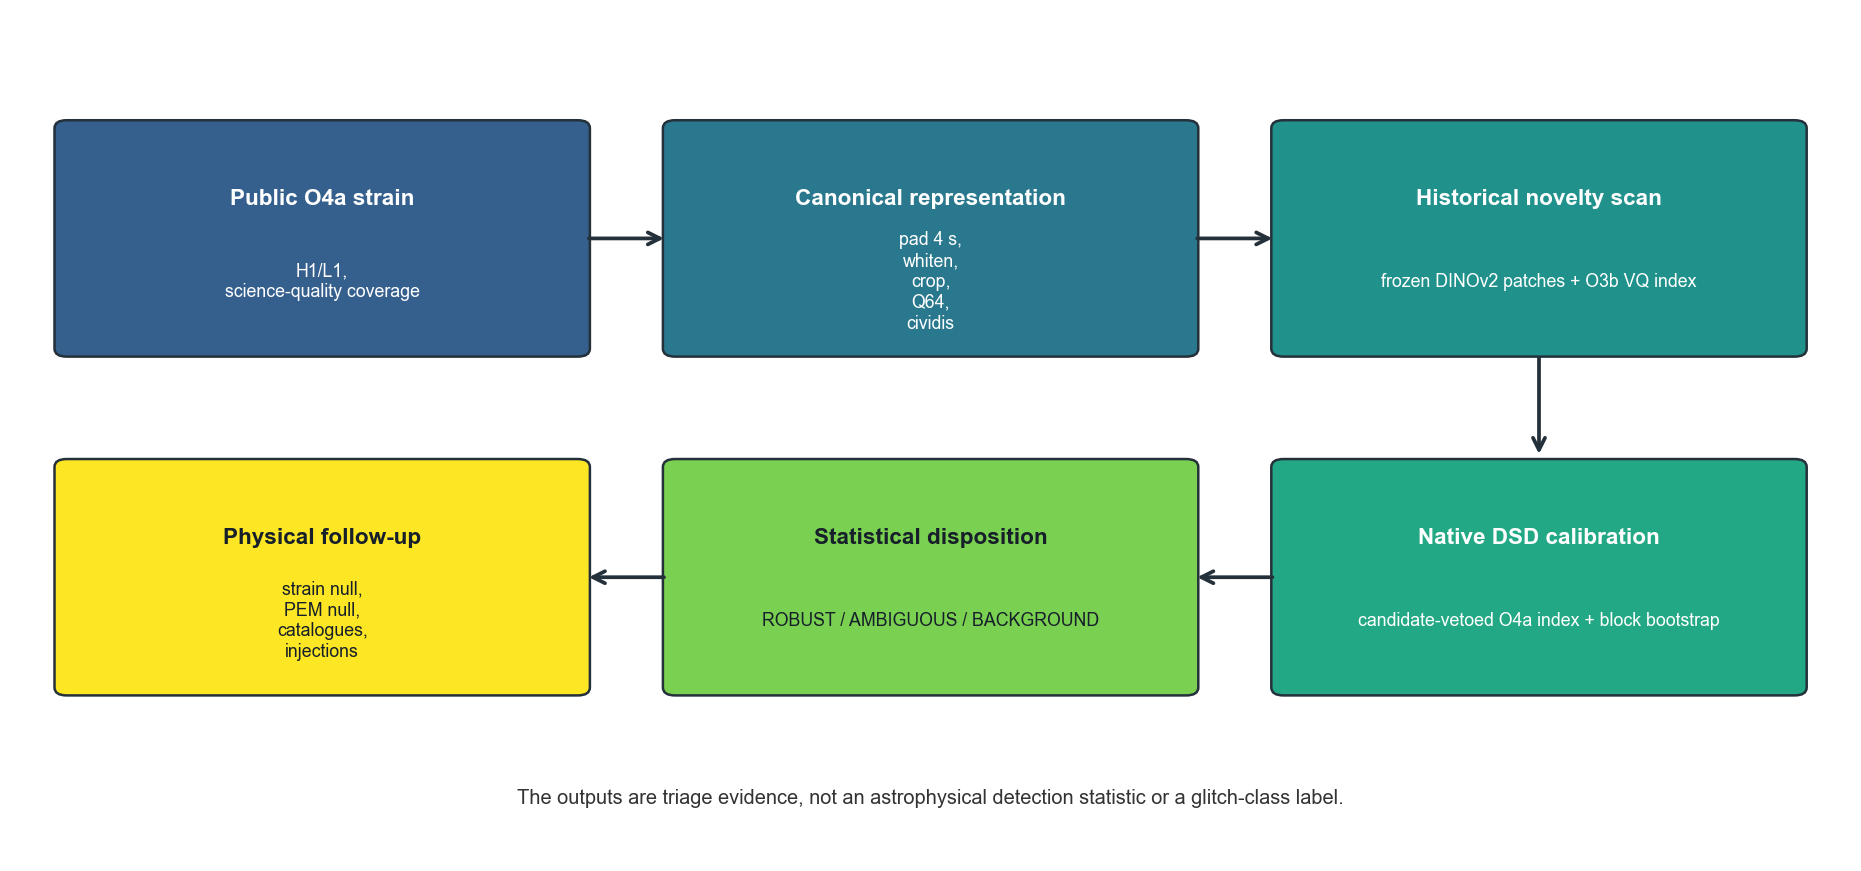
\includegraphics[width=0.96\textwidth]{fig_pipeline_overview.png}
\caption{End-to-end DANTE workflow used in this study.  The historical and
run-native reference populations are distinct; all arrows denote recorded
data products with representation and provenance checks.}
\label{fig:pipeline}
\end{figure*}

\subsection{Preprocessing and patch representation}

Each candidate is represented by a 32\,s analysis window at 4096\,Hz.  Strain is fetched
with 4\,s of context on each side, whitened on the padded interval, cropped back
to the clean subwindow, and band-passed once.  At this sample rate the configured
20--2000\,Hz passband is capped at 1843.2\,Hz to remain below Nyquist.  The
production DSD Q-transform requests $Q\in[4,64]$ and 20--2048\,Hz; for this
window and Q range GWpy lowers the effective logarithmic frequency axis to
20--1291.05\,Hz.  The resulting time-by-frequency array is resized without
transposition to a $256\times256$ cividis image.  It is converted to RGB, resized to
$518\times518$, converted to a floating-point tensor, and normalized with
ImageNet channel means $(0.485,0.456,0.406)$ and standard deviations
$(0.229,0.224,0.225)$.  The frozen DINOv2 ViT-S/14 encoder with registers maps
the image to 1,369 normalized 384-dimensional patch tokens.  The pipeline uses
patch tokens, not the global class token: prior work established that global
CLS-token pooling averages out short-duration transients occupying a small
fraction of the patch grid \cite{cirfeta2026patch}, a signal dilution effect that
prevented recovery at the calibrated operating point across the finite SNR
range tested in that study.

For normalized patch token $\mathbf z_j$ and normalized reference centroids
$\mathbf c_\ell$, the patch distance is
\begin{equation}
 d_j = \min_\ell \left(1-\mathbf z_j^\mathsf{T}\mathbf c_\ell\right).
\end{equation}
Let $\mathcal T_k$ denote the $k=68$ largest patch distances.  The
multiple-instance anomaly score is
\begin{equation}
 A(\mathbf x)=\frac{1}{k}\sum_{j\in\mathcal T_k}d_j .
\label{eq:mil}
\end{equation}
All saliency maps and stored MIL vectors use these same selected patches.
Figure~\ref{fig:representation} illustrates this exact representation path for
the retained L1 window used in the candidate-level reassessment.

\begin{figure*}[t]
\centering
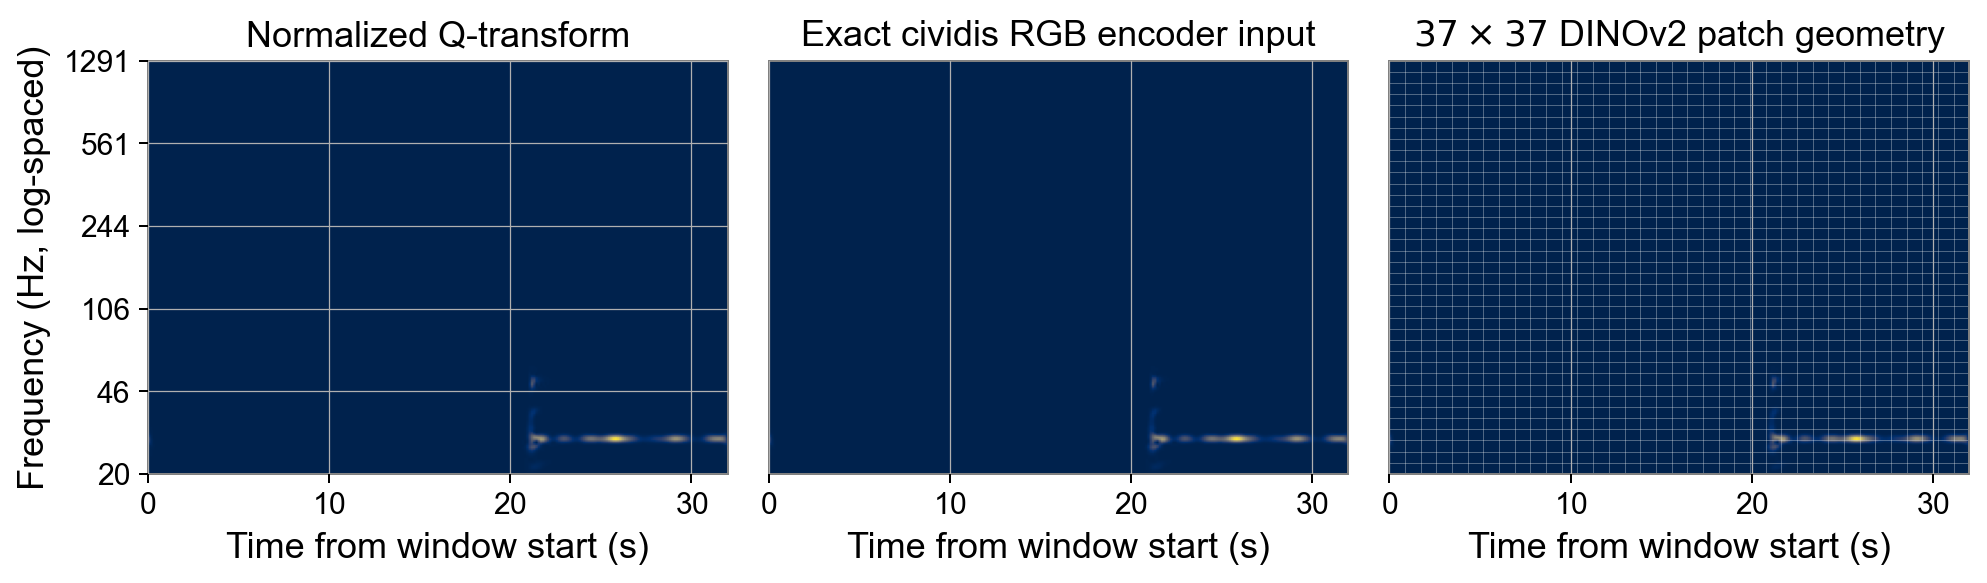
\includegraphics[width=0.96\textwidth]{fig_representation_examples.png}
\caption{Exact representation path illustrated with the retained L1 window at
catalogue GPS 1382955228.  The normalized time--frequency array (left) is
rendered with cividis before DINOv2 normalization (centre); the encoder then
produces a $37\times37$ patch-token grid (right).  Display transposition is
only for conventional time-horizontal plotting and is not applied to the
encoder input.}
\label{fig:representation}
\end{figure*}

\subsection{Primary candidate generation}

The primary scan partitions each available strain file into non-overlapping
32\,s windows.  For each session and detector, the O3b-dictionary novelty
threshold is the empirical $P_{99}$ of a seeded background sample, and a window
is retained when its Top-$k$ score exceeds that threshold.  The target sample
size is 500.  Of the 84 session--detector production files, 79 contain all 500
calibration windows; three contain 128, one 49, and one 38.  Consequently the
initial candidate-selection quantile has unequal finite-sample precision and
must not be interpreted as a uniform survey-wide 1\% false-positive rate.
This primary selection is distinct from the later 5,000-window DSD
calibration.  Consequently, every downstream result is conditional on this
O3b-novel candidate universe: the study does not evaluate O4a windows that are
rare relative to an O4a-native reference but remain below the historical O3b
selection threshold.

The scan produces 10,899 threshold exceedances (4,491 H1 and 6,408 L1).
A production geometry check removes 160 L1 windows whose selected Top-$k$
patches are centred in the outermost image columns and labels them suspected
edge artefacts.  The remaining 10,739 rows contain repeats where overlapping
macro-sessions score the same detector--time window.  Exact deduplication on
$(\mathrm{detector},\mathrm{GPS})$ removes 310 such rows and yields the 10,429
catalogue entries.  H1 and L1 records at the same GPS are retained as distinct
measurements.

The historical O4a production files also predate a timestamp-label correction:
their stored GPS marks the padded fetch start, 4\,s before the 32\,s interval
actually scored.  All retrospective rescoring therefore applies the declared
$+4$\,s offset; new scans store the analysis-window start directly.  Reuse of
the 10,372 pre-existing native scores is accepted only after exact
detector--GPS, representation, index-hash, offset, uniqueness, and finite-value
checks.  An independent forward pass from strain reproduces 60 retained stored
scores with maximum $|\Delta A|=6.85\times10^{-7}$, providing a numerical
check in addition to provenance matching.  The 57 detector-aware restored
windows are scored normally.

\subsection{Coherent native calibration}

A representation-contract ablation compares a $Q_{\max}=32$ native index
queried by $Q_{\max}=64$ candidate images with the coherent configuration in
which both use $Q\in[4,64]$.  The coherent configuration is the only one used
for downstream inference.  The index path, SHA256, Q-range, embedding
dimension, and normalization contract are stored with each dependent
artefact. All 10,429 candidates completed coherent scoring; none was silently
dropped. Exactly 10,372 scores were reused after detector--GPS and hash
verification and 57 were newly computed. Within the paired historical
population, the ablation changes 4,676 dispositions, demonstrating that
index/query representation is part of the statistical model rather than
metadata hygiene.

The coherent native dictionary is fit with MiniBatchKMeans \cite{sculley2010}
($K=1216$, batch size 4096, random seed 42) to 1,294 clean segments sampled
across H1 and L1.  Candidate windows and a 96\,s guard on either side are
excluded before sampling.  Centroids and query tokens are L2-normalized, and a
seeded 50,000-token pre-quantization sample is retained for perturbation tests.

For each detector, 5,000 chronological background windows are selected inside
the O4a bounds with zero candidate/guard or index-training overlap.  Scores are
partitioned into non-overlapping temporal blocks of 17 windows
\cite{kunsch1989}.  Resampling those complete blocks with replacement using
$B=10^6$ and seed 42 yields a percentile confidence interval
$[\tau_{\rm lo},\tau_{\rm hi}]$ for the background $P_{99}$.  We define
\begin{align}
 A &> \tau_{\rm hi} &&\Rightarrow \robust,\\
 \tau_{\rm lo}\le A\le\tau_{\rm hi} &&\Rightarrow \ambiguous,\\
 A &< \tau_{\rm lo} &&\Rightarrow \background.
\end{align}
The calibrated values are
\begin{align}
\mathrm{H1}:&(P_{99},\tau_{\rm lo},\tau_{\rm hi})
  =(0.16158,0.13023,0.20409),\\
\mathrm{L1}:&(P_{99},\tau_{\rm lo},\tau_{\rm hi})
  =(0.17606,0.15032,0.21959).
\end{align}
Repeating the complete $B=10^6$ calibration ten times gives endpoint Monte
Carlo standard deviations no larger than $4.89\times10^{-5}$; the H1 upper and
L1 lower endpoints are identical in all ten repeats.  The largest Monte Carlo
standard deviation is $7.1\times10^{-4}$ of its confidence-interval width.

The production length is the deterministic rule
$b=\lfloor n^{1/3}\rfloor=17$, not an estimate optimized on candidate labels.
We nevertheless audit this modelling choice with 200,000 replicas at
$b\in\{8,17,32,64\}$.  Relative to the released taxonomy, non-overlapping
blocks change 46, 1, 42, and 140 of 10,429 dispositions, respectively.  An
overlapping moving-block construction changes 86, 43, 7, and 148.  Thus at
least 98.58\% of the complete catalogue retains its disposition throughout
this grid, while up to 1.42\% of boundary cases remain block-model dependent.
This sensitivity is reported rather than folded into a post-hoc choice of
production threshold.
Table~\ref{tab:contracts} summarizes the populations, independence relations,
and representation contracts used throughout the analysis.

\begin{table}[htbp]
\centering
\caption{Populations and contracts used in the representation-coherent
analysis.  ``Independent'' means that candidate windows are not reused in the
listed calibration population.}
\label{tab:contracts}
\small
\begin{tabularx}{\textwidth}{lXr}
\toprule
Object & Construction and role & Size \\
\midrule
Primary O3b dictionary & Historical novelty reference; normalized
384-dimensional centroids & $K=275$ \\
Native O4a dictionary & Candidate-vetoed H1/L1 background; Q64; used by DSD
& $K=1216$ \\
Raw native-token sample & Pre-quantization tokens retained for point-level
controls & 50,000 \\
Threshold backgrounds & Independent chronological O4a windows, one population
per detector & $2\times5,000$ \\
Candidate catalogue & Unique H1/L1 detector--time windows after exact-repeat deduplication
& 10,429 \\
PEM validation sample & Score-rank-spaced coherent classes; all calibrated
& 141 \\
CBC controls & Three measured systems, five distances, 25 completed trials per
cell & 375 \\
\bottomrule
\end{tabularx}
\end{table}

\subsection{Physical and catalogue nulls}

Cross-detector coincidence is evaluated in whitened strain, not in embedding
space.  We maximize the normalized H1--L1 cross-correlation over the
inter-site light-travel interval plus a 2\,ms margin.  For each event we retain
the maximum over 4--8 valid time shifts; pooling these per-event maxima gives
$P_{99}$ threshold $\tau_{\rm cc}=0.4046$.  Among 8,806 evaluable candidate
windows, 13 single on-source values exceed this threshold.  Because an
on-source statistic is a single value whereas its null contribution is a
per-event maximum, this conservative screen is not an exchangeable tail-count
test and the 13/8,806 count is not assigned a $p$-value or a physical
interpretation.  The remaining 1,623 historical candidates have no validated
measurement; this missingness is not assumed random.  Relative to the 8,806
measured candidates, the unmeasured subset has nearly identical detector
composition (41.7\% H1 versus 42.4\%), a modestly smaller \robust\ fraction
(58.0\% versus 61.6\%), and a lower median native score (0.327 versus 0.398),
while the score $P_{99}$ is similar (0.494 versus 0.496).  Thus the missing
subset is not distributionally identical, but it is not selectively depleted
in the extreme score tail.

For environmental coupling, magnitude-squared coherence is calculated with
Welch's method \cite{welch1967} across the public auxiliary channels available
for each event.  The primary endpoint requires the observed family-wise maximum
to exceed both an event-specific time-shift $P_{99}$ and a quiet-background
zero-lag $P_{99}$.  This second null is necessary because persistent spectral
coherence can make time shifts alone non-discriminating.  Channels in the
public release are not treated as safety-certified veto channels.

For each event, the family-wise time-shift null is drawn from a nearby 4\,h
CAT1-clean block after excluding 96\,s around every catalogue candidate.
Magnitude-squared coherence uses 2\,s Welch segments with 1\,s overlap over
20--500\,Hz.  Thirty-two-second windows are separated by a 96\,s stride, and
all ordered strain--auxiliary window pairs separated by at least 64\,s enter
the null.  The same time shift is applied to all available channels so that
their cross-channel dependence is preserved.  The event statistic is the
maximum over channel and frequency; its family-wise level is $\alpha=0.01$.
Threshold uncertainty is bootstrapped over window indices, not over dependent
window pairs.  The quiet-background control uses the $P_{99}$ of the zero-lag
maxima from those candidate-free windows.

Catalogue overlap uses GWTC-4.0/4.1 event times falling in the O4a interval
\cite{gwtc4_results,gwtc41_release}.
Because the historical scan did not persist an exact successful-window ledger,
raw block coverage is an upper-bound proxy.  The null circularly shifts the
complete catalogue by 10,000 common offsets of at least one day, preserving
its internal temporal structure.

\section{Results}
\label{sec:results}

\subsection{Detector-dependent domain shift and known-glitch controls}
\label{sec:domain-known}

We first test the premise for native adaptation directly, before examining the
O4a candidate taxonomy.  For each detector, 100 vetoed clean windows from O3b
and 100 from O4a are split chronologically into 60 dictionary-training and 40
held-out windows.  We set the dictionary size by the same compression-density
rule used for the production native index: each training pool contains
$60\times1369$ patch tokens, and 1,458 tokens per centroid gives matched $K=56$
O3b and O4a dictionaries after rounding.  The smaller absolute $K$ therefore
tracks the smaller training pool and is not, by itself, evidence of stronger
compression.  This construct-control size is nevertheless distinct from the
production O3b ($K=275$) and native O4a ($K=1216$) dictionaries; the
score-based cross-run endpoints remain conditional on these samples and the
$K=56$ control.  The fixed O3b control dictionary gives an H1 mean
O4a-minus-O3b score
difference of $0.03983$ (95\% bootstrap interval
$[0.02914,0.05184]$; two-sample KS $p=1.23\times10^{-7}$).  Replacing that
dictionary with its O4a-native counterpart lowers the paired H1 O4a score by
$0.02737$ on average ($[-0.03296,-0.02158]$).  A five-block out-of-fold probe,
computed from L2-normalized segment-mean embeddings without either $K=56$
dictionary, also separates the H1 runs with AUC $0.920$ ($[0.881,0.955]$).

The same endpoints do not support an analogous L1 claim.  The L1 O4a-minus-O3b
difference is $-0.00290$ ($[-0.01304,0.00823]$; KS $p=0.097$), and the paired
native-minus-cross-index change is $0.00035$ ($[-0.00513,0.00582]$).  The L1
run-probe AUC is $0.616$ ($[0.535,0.694]$).  The motivation and effect of
native adaptation are therefore detector-dependent in these samples, rather
than a universal property of O4a (Fig.~\ref{fig:domain-known}a--c).

As an external construct control, the same O3b dictionaries score 30
Gravity-Spy-labelled examples \cite{gspy_zenodo} of each of Blip, Scattered Light, and Koi Fish
per detector against 40 held-out clean O3b windows.  DANTE AUCs are
$0.670$, $1.000$, and $1.000$ for H1, and $0.523$, $0.988$, and $0.993$ for
L1, respectively.  The Blip intervals are broad and include weak separation:
$[0.536,0.791]$ for H1 and $[0.382,0.663]$ for L1.  These are binary,
morphology-specific O3b controls, not O4a multiclass recall or evidence that
all known glitches are discovered (Fig.~\ref{fig:domain-known}d).  In
particular, the weak L1 Blip result is a material construct-validity limit for
short broadband transients.  The present experiments do not identify its
cause or establish that it shares a mechanism with the low-$Q$ injection blind
region; neither patch pooling nor the frozen natural-image representation is
therefore assigned a causal explanation here.

\begin{figure*}[t]
\centering
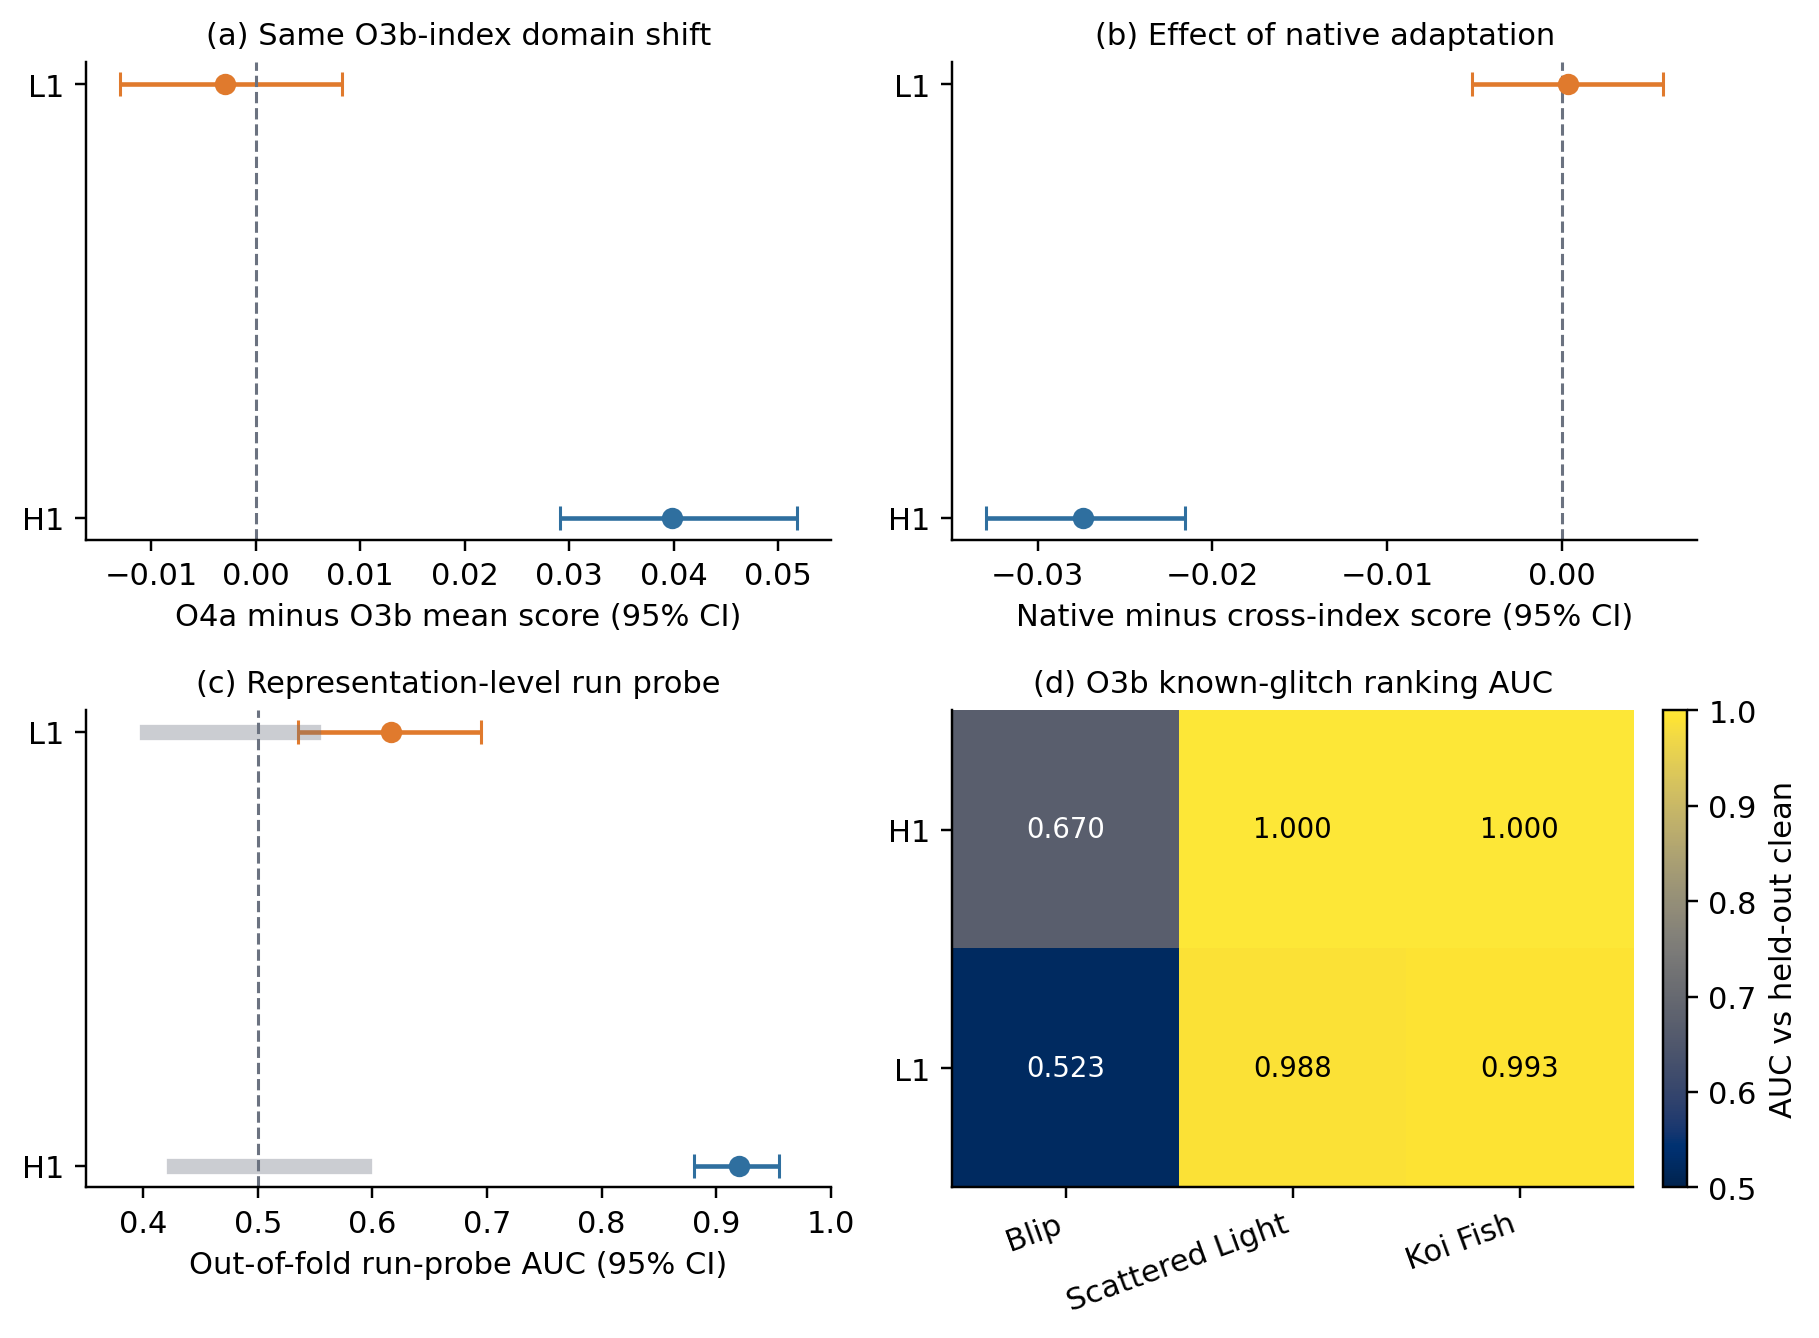
\includegraphics[width=0.94\textwidth]{fig_domain_known_q64.png}
\caption{Direct domain and known-glitch controls under the coherent Q64
representation.  (a) Held-out score difference between O4a and O3b using the
same O3b index.  (b) Paired O4a score change after native adaptation.
(c) Out-of-fold run-probe AUC.  Points and bars in (a--c) are estimates and
95\% bootstrap intervals.  (d) Binary AUC for three O3b Gravity Spy
morphologies against held-out clean strain; each cell uses 30 labelled and 40
clean windows.}
\label{fig:domain-known}
\end{figure*}

\subsection{Discovery disposition is not physical classification}

The coherent taxonomy contains 6,365 \robust, 1,275 \ambiguous, and 2,789
\background\ windows (Fig.~\ref{fig:funnel}).  Detector-specific \robust\
fractions are 50.5\% for H1 and 68.8\% for L1. These labels state where a
score lies relative to a run-native background interval.  They do not by
themselves identify a glitch family, an instrumental cause, or an
astrophysical signal.

\begin{figure}[t]
\centering
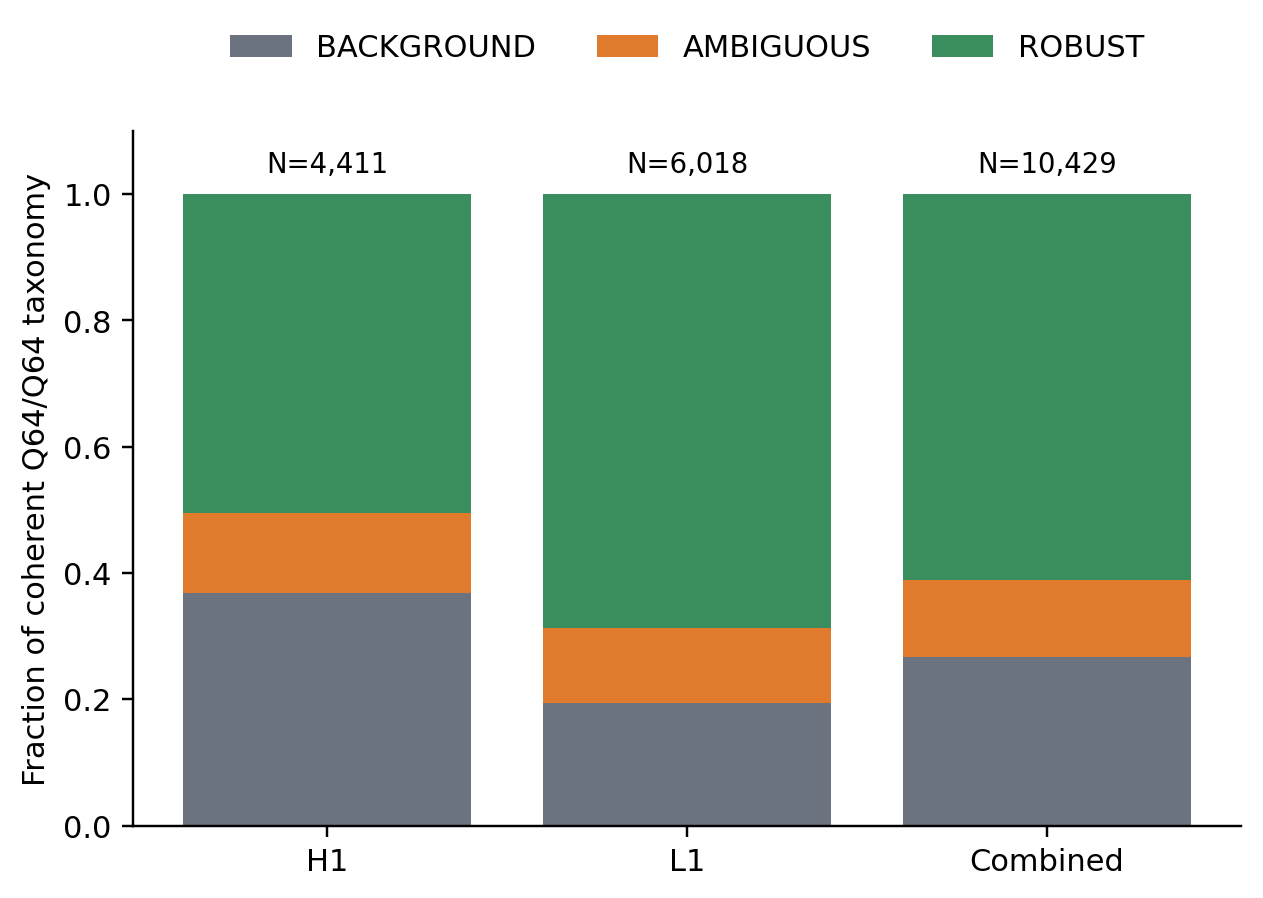
\includegraphics[width=\columnwidth]{fig_funnel_q64.png}
\caption{Coherent Q64/Q64 DSD disposition by detector and combined.  Counts
above each bar include every evaluated candidate.}
\label{fig:funnel}
\end{figure}

At the graph-distance cut $D_{\rm cut}=0.25$, fixed before the final execution, the topology is
saturated. The largest connected component contains 99.92\% of \robust\
candidates and 100\% of \ambiguous, \background, and 3,000 unselected
native-background vectors.
Identical clustering therefore does not distinguish anomaly status.  Likewise,
the strongest cross-session pairs occur at approximately the all-pairs
cross-session rate, and the mean neighbour-session span is below a shuffled
session null.  The current embedding resolves no positive recurrence signal;
this is not evidence that no physical morphology recurs.

\subsection{Sensitivity of the statistical disposition}

The C2 stress test uses four independent 1,300-segment native-background draws
and gives mean pairwise
Spearman correlation $\rho=0.674$ and minimum $0.515$ for a deliberately
near-boundary sample of 80 \robust\ and 80 \ambiguous\ candidates
(Fig.~\ref{fig:robustness}a).  The median per-candidate score standard
deviation is 0.00757. Candidate ordering is positively, but only moderately,
stable to the background draw.

Dictionary size also matters (Fig.~\ref{fig:robustness}b).  Relative to
$K=1216$, rank correlation is 0.753, 0.768, and 0.943 for
$K=512,1024,2048$, respectively.  Ranking becomes more similar near and above
the production size but is not invariant to $K$.  As simple alternatives, a
PCA reconstruction residual and total spectral energy yield AUC 0.436 and
0.544 for separating the same coherent classes, and correlations $-0.158$ and
$0.030$ with DANTE (Fig.~\ref{fig:robustness}c). Energy AUC is
detector-dependent (0.598 for H1 and 0.490 for L1).  As a nonlinear
GW-specific control, we train a small convolutional autoencoder separately for
each detector on 650 candidate-vetoed O4a Q-transform backgrounds.  The input
is the same $32\times32$ log-power representation; an 8--16--16 channel encoder
maps to a 16-dimensional latent vector, and reconstruction error is converted
to a percentile of held-out detector background.  Across seeds 42, 314159 and
271828, the pooled AUC is 0.473 (seed range 0.473--0.485) and Spearman
correlation with DANTE is $-0.047$; H1/L1 AUC is 0.528/0.424.  This negative
control shows that nonlinear GW-specific reconstruction error does not
reproduce the DANTE disposition.  These comparators neither establish the
optimality nor assign causal morphological meaning to the natural-image
features.

The canonical 4\,s whitening-context implementation reproduces all 60 retained
anchor scores to a maximum absolute difference $6.85\times10^{-7}$.  Six of
66 attempted candidates are excluded by a hashed ledger for non-finite context
or anchor mismatch.  The retained near-boundary disposition is sensitive to
context (Fig.~\ref{fig:robustness}d).  Relative to pad 4\,s, fixed-threshold
flip fractions are 40.0\%, 40.0\%, and 36.7\% at pads 16, 64, and 128\,s;
after recalibrating 5,000 background windows per detector at every pad they are
63.3\%, 70.0\%, and 65.0\%. The median score swing is 0.0109 and 16/60 exceed
0.02. These are boundary-conditioned sensitivities, not
survey-wide failure rates.

A separate final replication study holds the candidate-token pools fixed and
varies one model component at a time (Fig.~\ref{fig:robustness-replicates}).
Across eight independent background draws, mean pairwise rank correlation is
$0.934$ ($[0.913,0.945]$; minimum pair $0.834$) for the near-boundary pool and
$0.977$ ($[0.962,0.984]$; minimum $0.929$) for an unconditioned 160-candidate
pool.  Across five MiniBatchKMeans seeds the corresponding means are $0.954$
($[0.936,0.963]$; minimum $0.896$) and $0.988$
($[0.978,0.992]$; minimum $0.981$).  Across
$K\in\{512,1024,1216,2048\}$ they are $0.903$
($[0.868,0.926]$; minimum $0.830$) and $0.978$
($[0.963,0.987]$; minimum $0.962$).  Thus the ranking is consistently more
stable in the unconditioned population; neither result justifies replacing
the C2 boundary-conditioned endpoint because the sampling and model ensembles
are different.

\begin{figure*}[t]
\centering
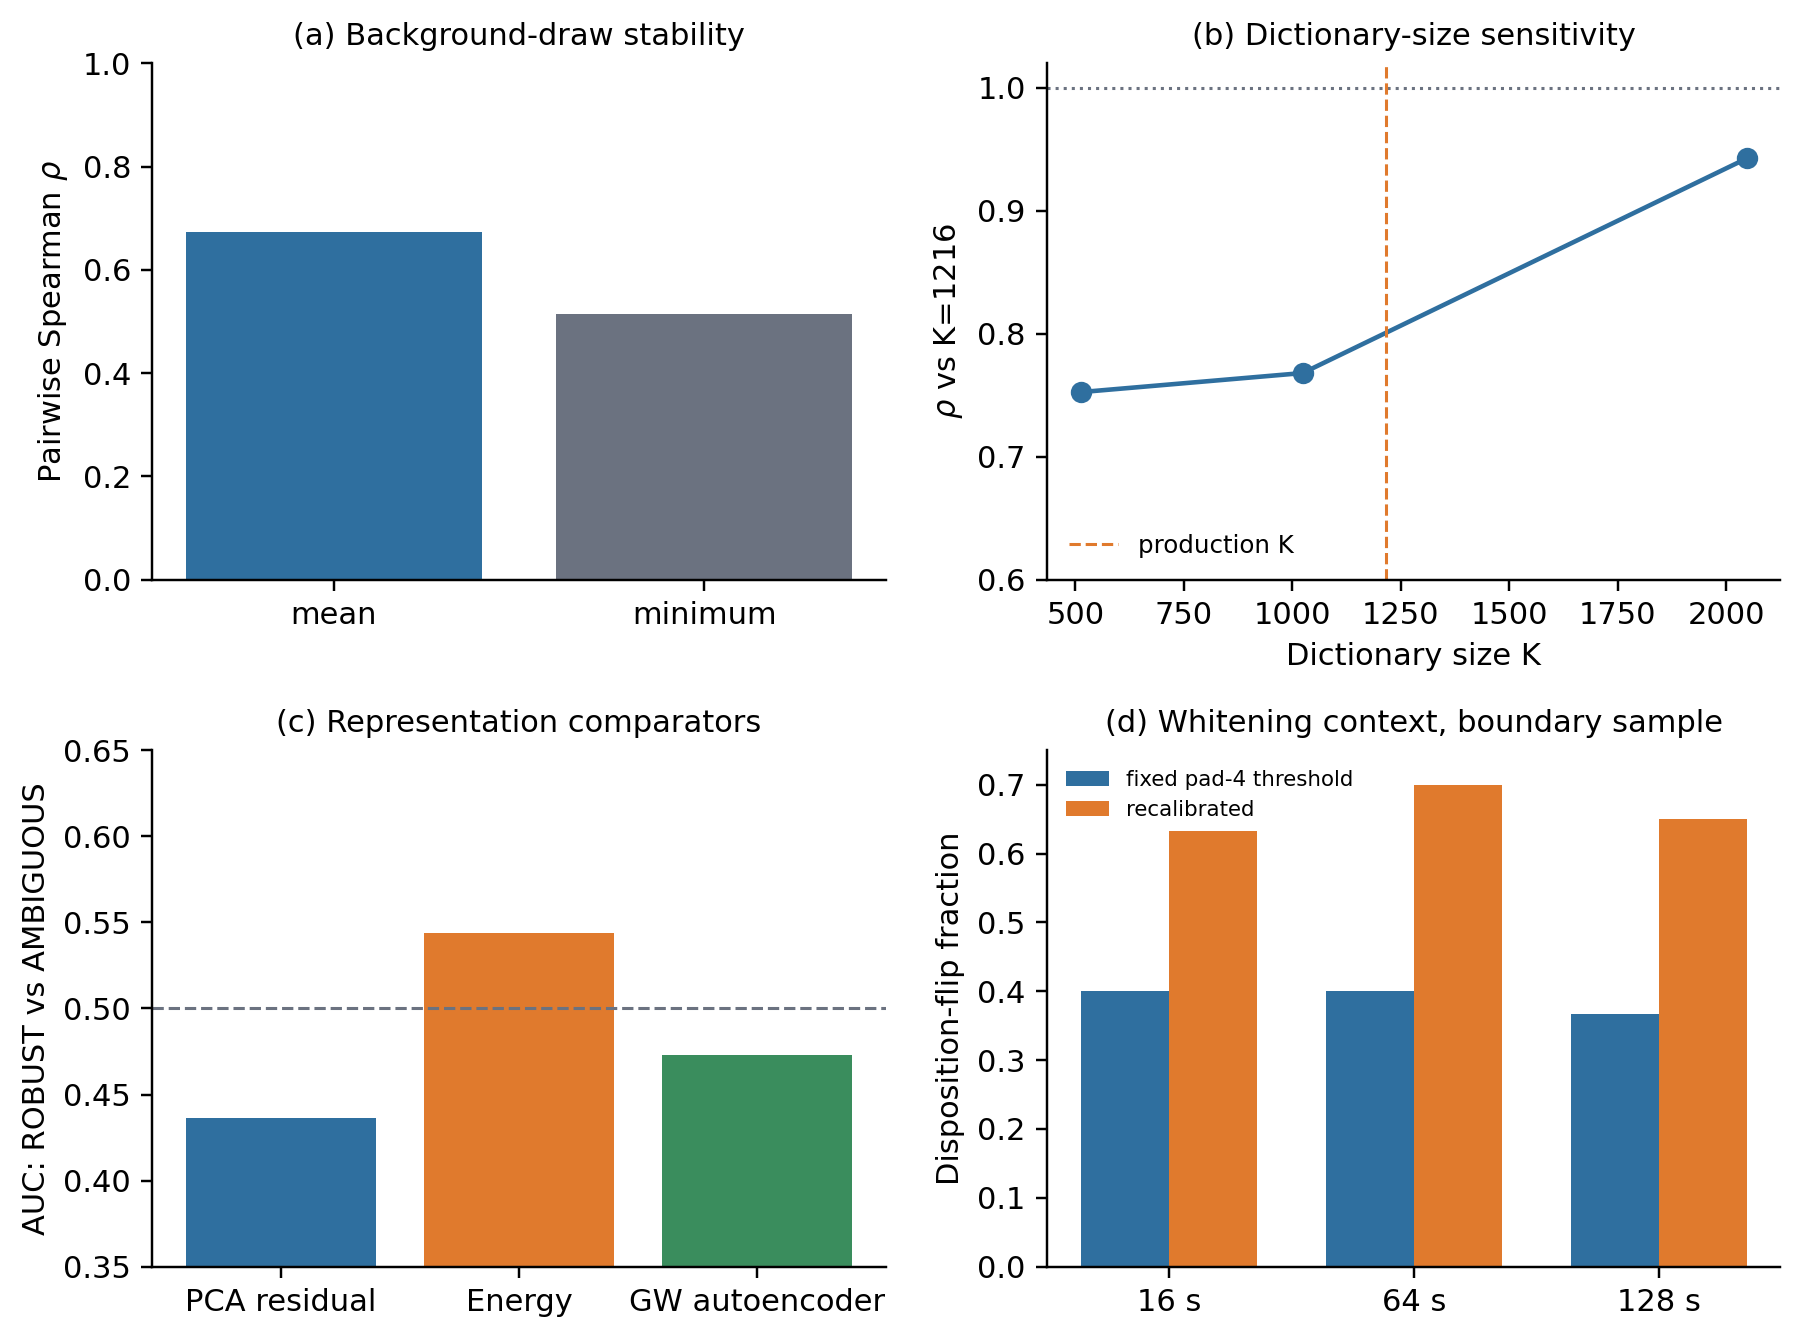
\includegraphics[width=0.92\textwidth]{fig_robustness_q64.png}
\caption{Sensitivity and baseline controls on representation-coherent,
near-boundary samples.  (a) Stability to native-background draw.  (b) Rank
correlation versus the production dictionary size.  (c) Classical pixel
baselines and a detector-specific GW-spectrogram autoencoder negative control.
(d) Candidate disposition under longer whitening contexts.}
\label{fig:robustness}
\end{figure*}

\begin{figure*}[t]
\centering
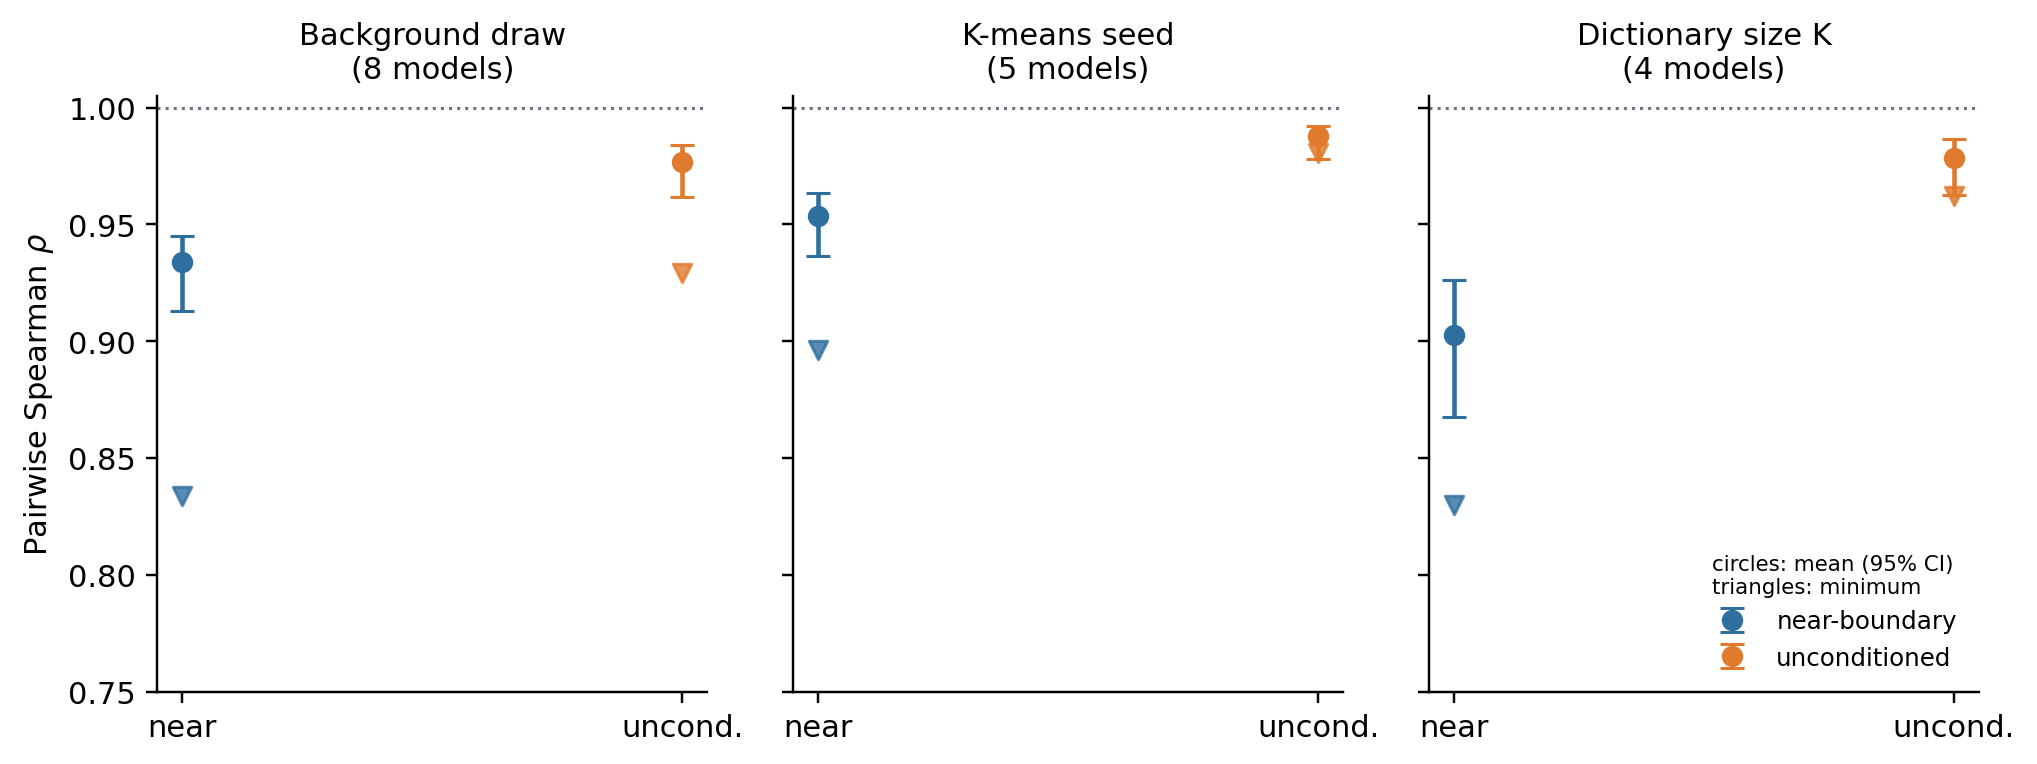
\includegraphics[width=0.92\textwidth]{fig_robustness_replicates_q64.png}
\caption{Final replicated robustness study.  Circles show the mean pairwise
Spearman correlation with 95\% candidate-bootstrap intervals; triangles show
the minimum observed pairwise correlation.  Near-boundary and unconditioned
candidate pools are reported separately for background draw, clustering seed,
and dictionary-size perturbations.}
\label{fig:robustness-replicates}
\end{figure*}

\subsection{Native adaptation can absorb recurrent anomalies}

We inject controlled Blip, Koi Fish, and Scattered Light morphologies at fixed
peak amplitude 12 in whitened-strain units and durations 1, 1, and 1.5\,s,
respectively, into increasing fractions
$\{0,0.02,0.05,0.10,0.15,0.20,0.30,0.40\}$ of a 300-segment O4a L1
native-index training set and evaluate 60 held-out injections.  Scaling the
production tokens-per-centroid ratio to this controlled sample gives $K=282$,
distinct from the production native index with $K=1216$.  Each morphology is
repeated with three clustering seeds.  An absorption crossing fixed before the
final replicated execution
requires both standardized injection/background separation $z\le3$ and a
held-out fraction above the index-specific background $P_{99}$ no larger than
0.5.

Each generated waveform is normalized to unit peak before scaling, added to a
whitened 32\,s segment at a seeded random position away from the filter edges,
and encoded through the same Q64 path.  Thus amplitude 12 is an SNR-like
whitened-noise scale, not a matched-filter SNR.  The 60 injected and 150
background evaluation segments are disjoint from both the 300 index segments
and the injected examples used to contaminate that index; a same-size
all-background dictionary controls the effect of changing the training-set
composition.

All seeds cross this joint rule: Blip at 2--5\% prevalence, Koi Fish at 10\%,
and Scattered Light at 5\% (Fig.~\ref{fig:absorption-matrix}).  At zero
contamination, median $z$ is 7.05, 18.13, and 21.61, respectively, while the
median flagged fraction is 0.717, 1.000, and 1.000.  Both endpoints fall with
contamination, whereas same-size all-background controls remain strongly
separated.  The experiment resolves the absorption mechanism across these
synthetic morphologies and seeds, but its crossing values remain conditional
on detector, amplitude, duration, sampling, representation, and rule.

\begin{figure*}[t]
\centering
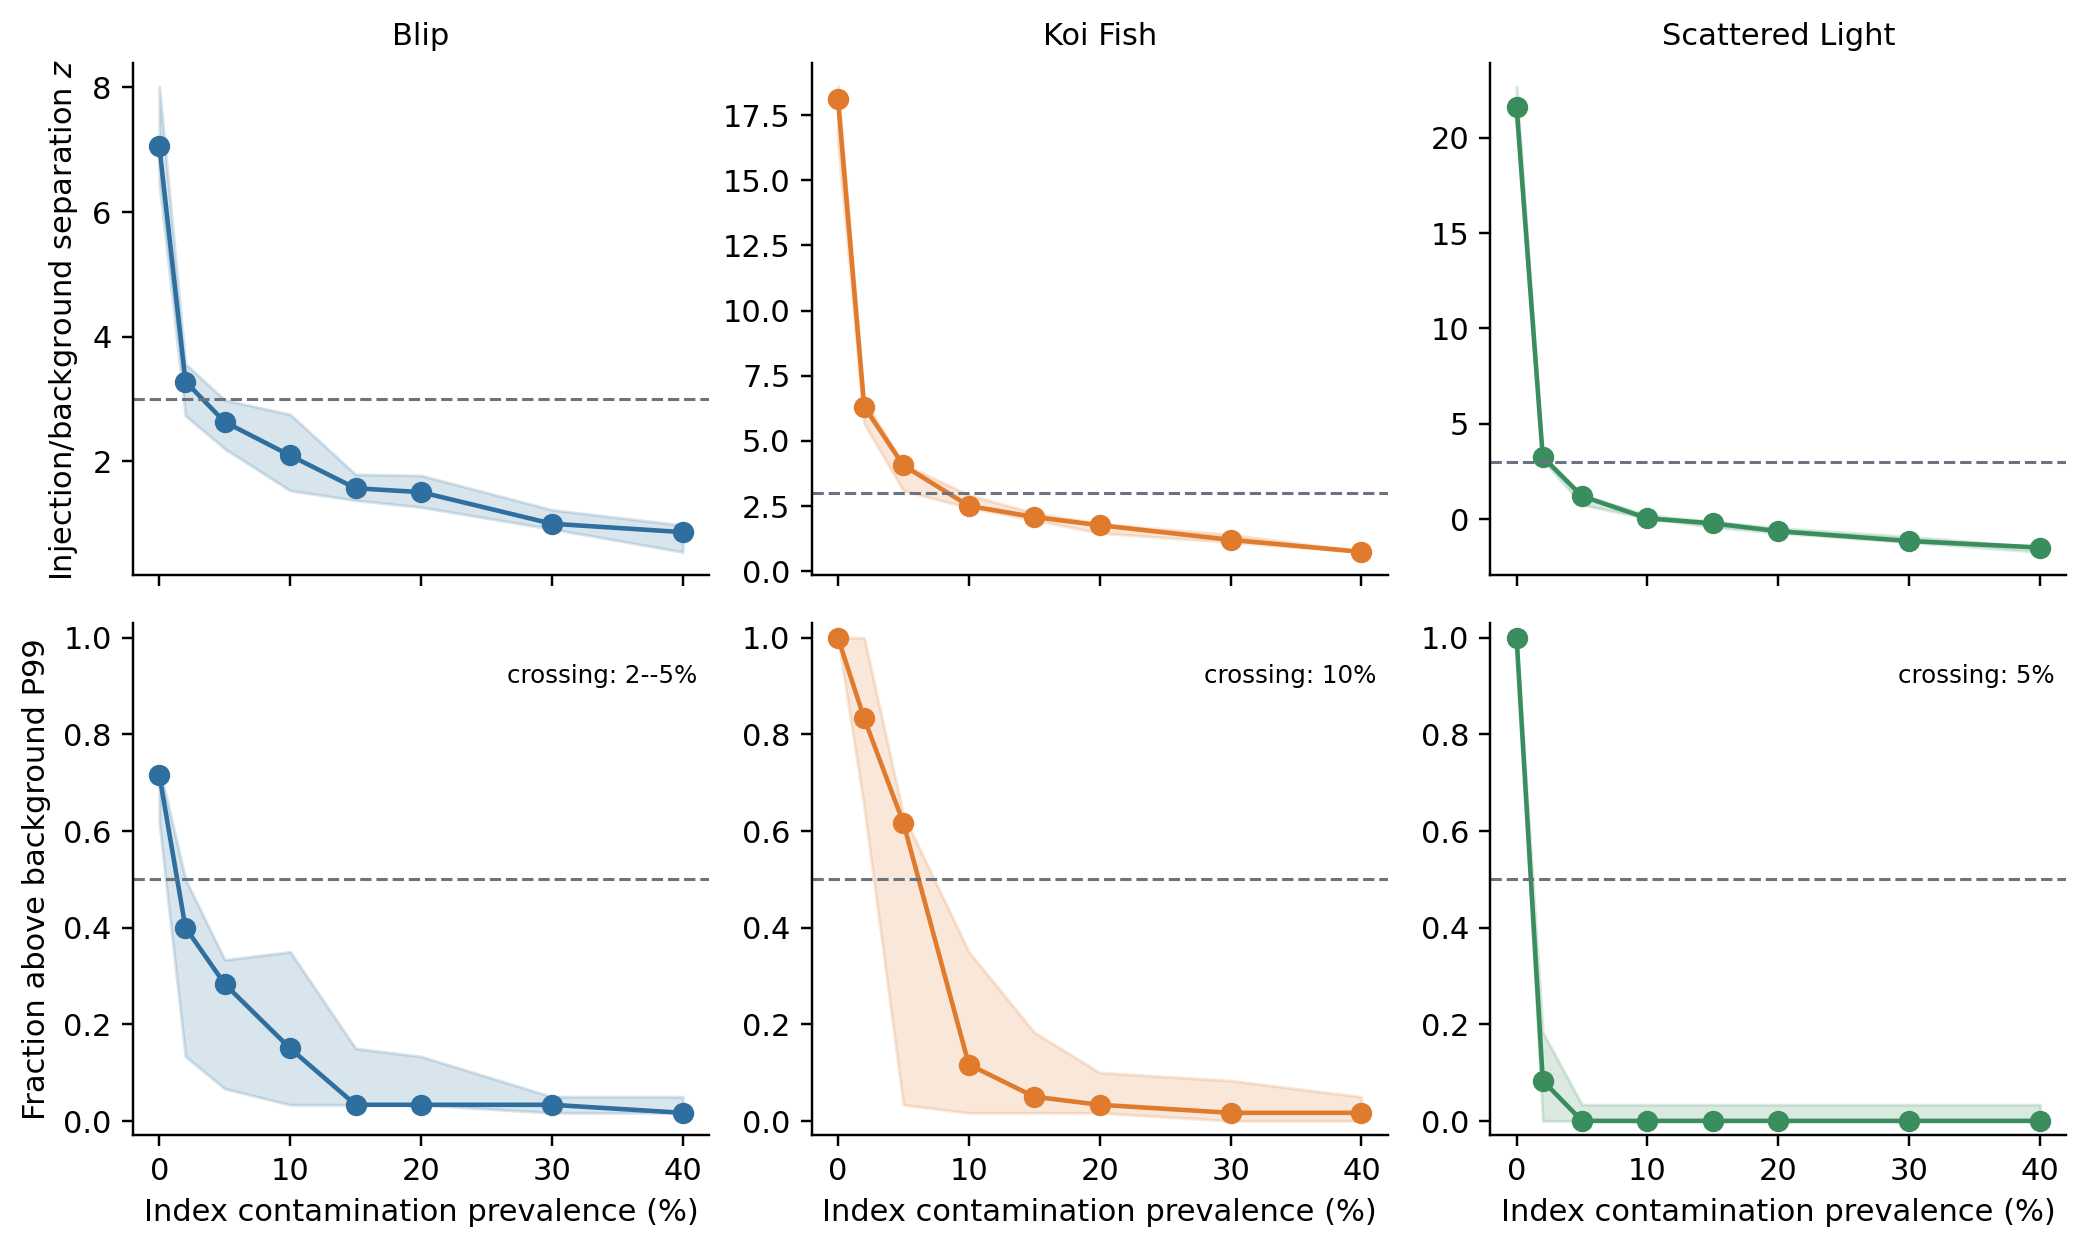
\includegraphics[width=0.94\textwidth]{fig_absorption_matrix_q64.png}
\caption{Controlled native-index absorption matrix for three injected
morphologies and three clustering seeds.  Lines show the across-seed median;
bands show the seed range.  Dashed lines mark the joint crossing rule
($z\le3$ and fraction above background $P_{99}\le0.5$).  The
300-segment, $K=282$ experimental dictionaries are distinct from the
$K=1216$ production native index.}
\label{fig:absorption-matrix}
\end{figure*}

\subsection{Empirical blind region}

A centred sine-Gaussian grid spans five frequencies, eight Q values, and eight
realizations per cell at fixed injected matched-filter SNR 20
(Fig.~\ref{fig:blind}).  For every clean 32\,s L1 segment, the waveform is
scaled using
\begin{equation}
 \rho^2=4\int_{20\,\mathrm{Hz}}^{2000\,\mathrm{Hz}}
 \frac{|\tilde h(f)|^2}{S_n(f)}\,\mathrm df,
\end{equation}
where $S_n$ is estimated from that same clean segment with 4\,s FFTs; the
waveform centre is then placed at the centre of the analysis window before the
canonical whitening and Q64 transform.  Mean
primary flag rate is 26.3\% for $Q\le64$ and 48.8\% for $Q>64$.  Every
$Q=2$ and $Q=4$ cell has zero recovery and most $Q=8$ cells also fail.  The
data reject a proposed universal loss of sensitivity above $Q_{\max}=64$ and
instead show a broad low-Q blind region with additional frequency-dependent
structure.  Individual-cell binomial intervals are wide because $n=8$.

\begin{figure}[t]
\centering
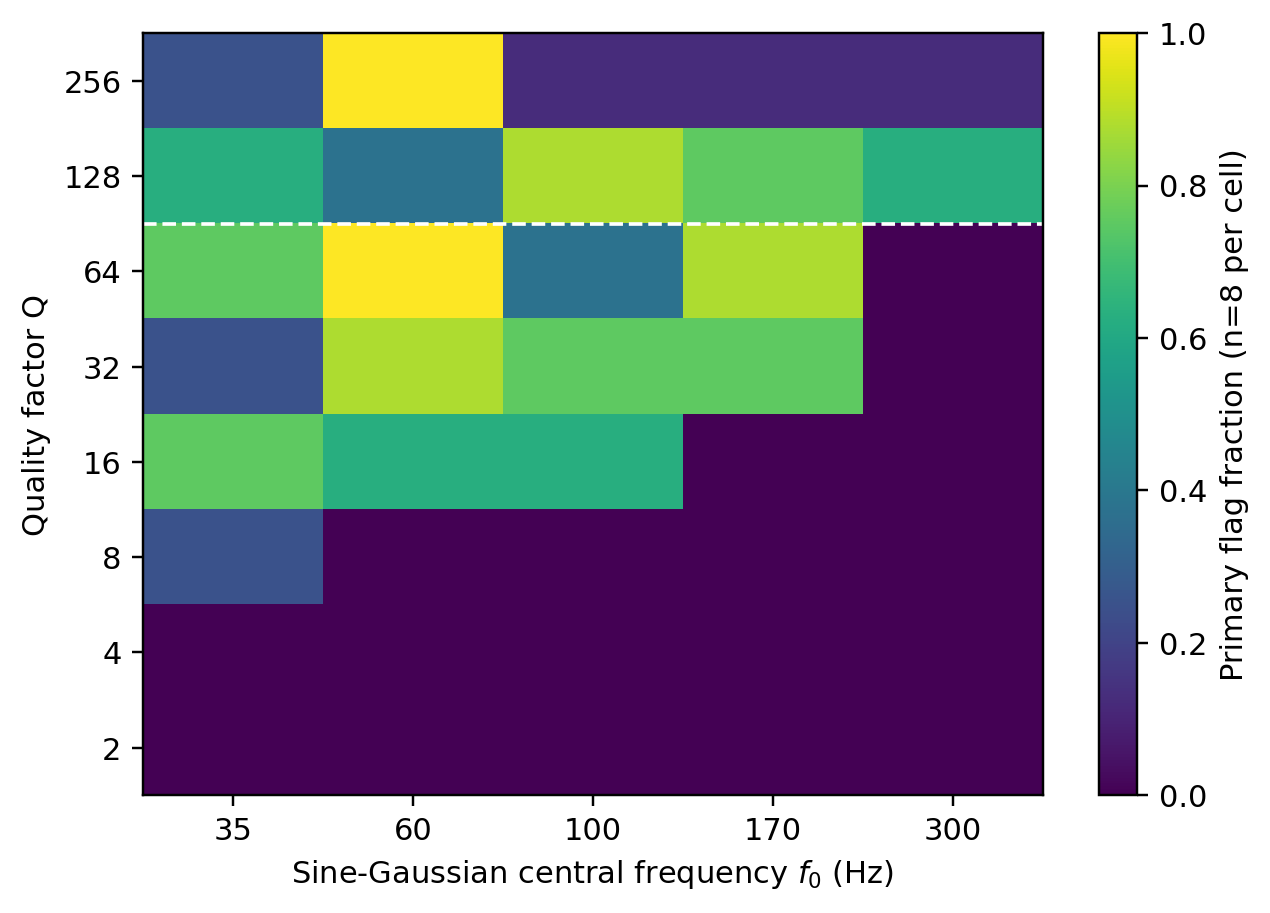
\includegraphics[width=\columnwidth]{fig_blind_spot_q64.png}
\caption{Primary flag fraction for centred sine-Gaussian injections at fixed
SNR 20.  The dashed line separates $Q\le64$ from $Q>64$; the dominant blind
region is at low Q, not uniformly above the representation boundary.}
\label{fig:blind}
\end{figure}

\subsection{Physical controls}

The PEM experiment uses a fixed measured cohort of 141 events originally
selected by spacing over score rank within the already coherent Q64/Q64
taxonomy.  Exact detector--GPS rejoining after a subsequent update of that
coherent taxonomy changes eight class labels and gives the current composition of 26
\robust, 22 \ambiguous, and 93 \background\ events.  Immutable event and null
measurements are reused only after their input hashes and keys match; this is
not a newly drawn class-balanced sample.  All 141 receive an empirical
family-wise calibration.  A time-shift threshold alone is not a coupling
endpoint: 6/26 \robust\ and 34/93 \background\ events exceed it (odds ratio
0.521, two-sided Fisher $p=0.245$), while 38 of the 48 exceedances fail the
quiet-background zero-lag control. The primary endpoint retains 2/26
\robust, 1/22 \ambiguous, and 7/93 \background\ events
(Fig.~\ref{fig:pem}); for \robust\ versus \background\ the odds ratio is
1.02 with two-sided Fisher $p=1.000$. Thus the coherent sample does not
resolve class enrichment in auxiliary coupling.  The point estimate is not
evidence of equal rates, and the public-channel inventory does not exclude
unmeasured couplings.

\begin{figure}[t]
\centering
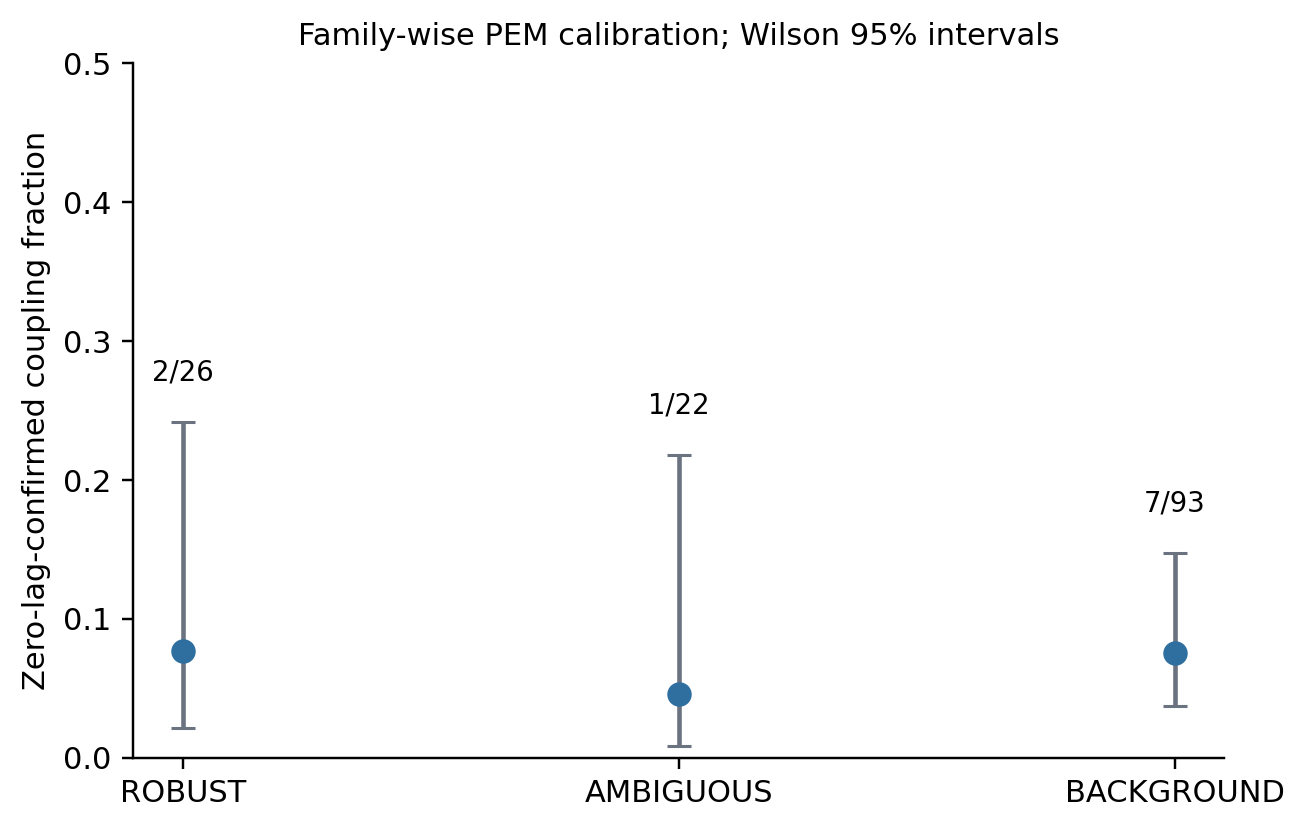
\includegraphics[width=\columnwidth]{fig_pem_q64.png}
\caption{Primary family-wise PEM endpoint with Wilson 95\% intervals
\cite{wilson1927}.
All 141 selected events are calibrated; the intervals remain broad for the
smaller coherent classes.}
\label{fig:pem}
\end{figure}

\subsection{A retained candidate is not a discovered class}

To make the distinction between statistical and physical evidence concrete,
we revisit the L1 entry at catalogue GPS 1382955228.  Historical timestamps
label the padded crop, so its exact analysis interval is GPS
1382955232--1382955264 and the localized feature occurs at GPS
1382955253.17.  The current native score is 0.598877 and its DSD disposition
is \robust.  Figure~\ref{fig:candidate} was regenerated through the canonical
pad-4, Q64, cividis, DINOv2 and native-index path; its Top-68 mean reproduces
the taxonomy value to $1.2\times10^{-7}$.

\begin{figure*}[t]
\centering
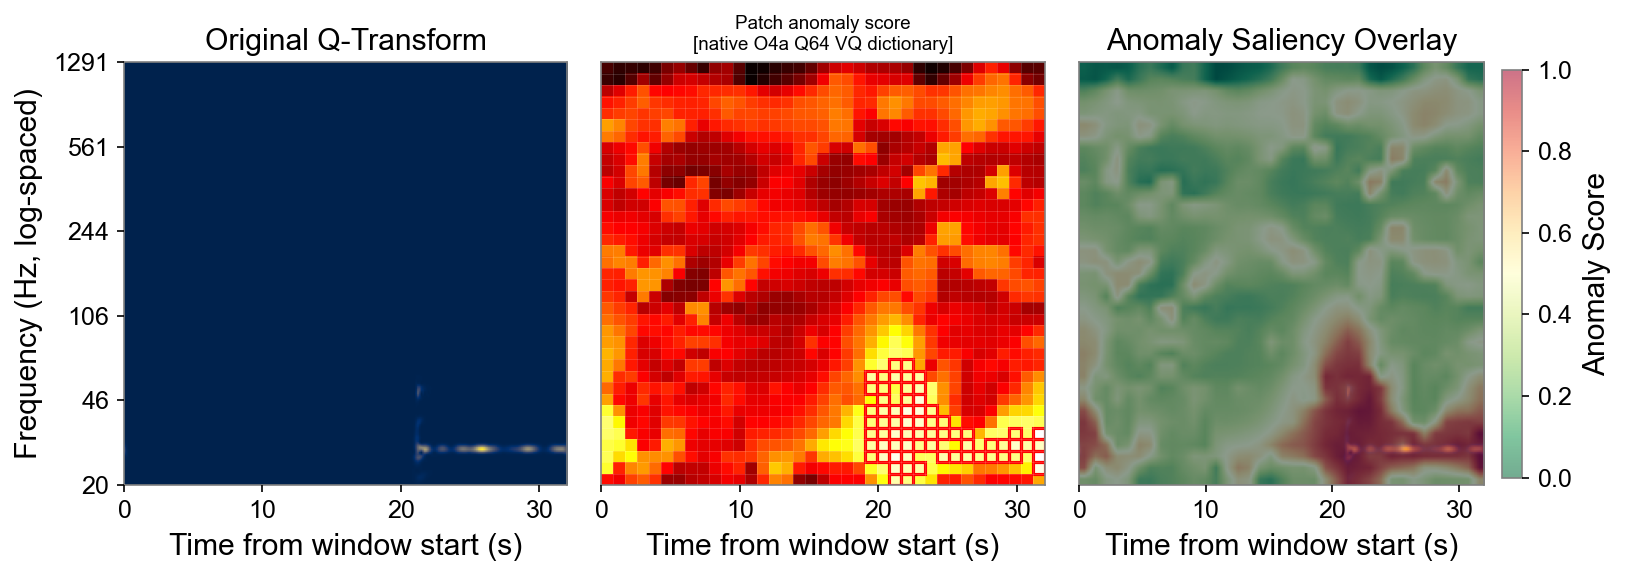
\includegraphics[width=0.96\textwidth]{fig_candidate_saliency_q64.png}
\caption{Canonical coherent-Q64 view of the retained L1 candidate.  Red boxes
are the production Top-68 native-index patches pooled into the DSD score.  The
map localizes statistical distance from the native dictionary; it is not a
morphology classifier or a causal map.}
\label{fig:candidate}
\end{figure*}

An independently implemented descriptive recipe, adapted from a public
proposal by Kretski and archived with the versioned analysis code and evidence
bundle \cite{dante_zenodo,dante_v6_evidence},
finds a peak near 28 Hz and in-band energy 304 times the mean of 16 adjacent
windows.  The event exceeds its scale-specific $P_{99}$ threshold at 0.5, 1,
2, and 4 s, with the largest margin (0.112) at 4 s.  These observations support
a loud, low-frequency L1-local transient.

The physical controls do not supply a classification.  The on-source H1--L1
coincidence coefficient is 0.0716, below the seven-shift null mean 0.197 and
maximum 0.286; patch intersection-over-union is 0.0074.  The public-channel
PEM statistic is 0.478, below both the family-wise threshold 0.663 and quiet
zero-lag threshold 0.789.  No H1 counterpart or coupling in the tested public
auxiliary subset is therefore resolved.  Qualitative resemblance to
low-frequency scattered-light-like ringing is hypothesis-generating only.
The event remains unclassified and is not evidence for a new glitch class;
the limited PEM inventory cannot exclude an unmeasured instrumental coupling.

The catalogue control covers 131 of 135 O4a catalogue events in at least one
detector under the raw-block proxy and 118 in both.  Two H1 candidate windows
overlap a catalogue event and none overlap in both detectors.  Circular shifts
give $2.190\pm1.467$ expected any-detector overlaps, a 95\% interval $[0,5]$,
and empirical $p=0.651$.  This is no resolved overlap excess.  It is not a
recall measurement because exact historical processed-window coverage is
unavailable (Fig.~\ref{fig:catalog-null}).

\begin{figure}[t]
\centering
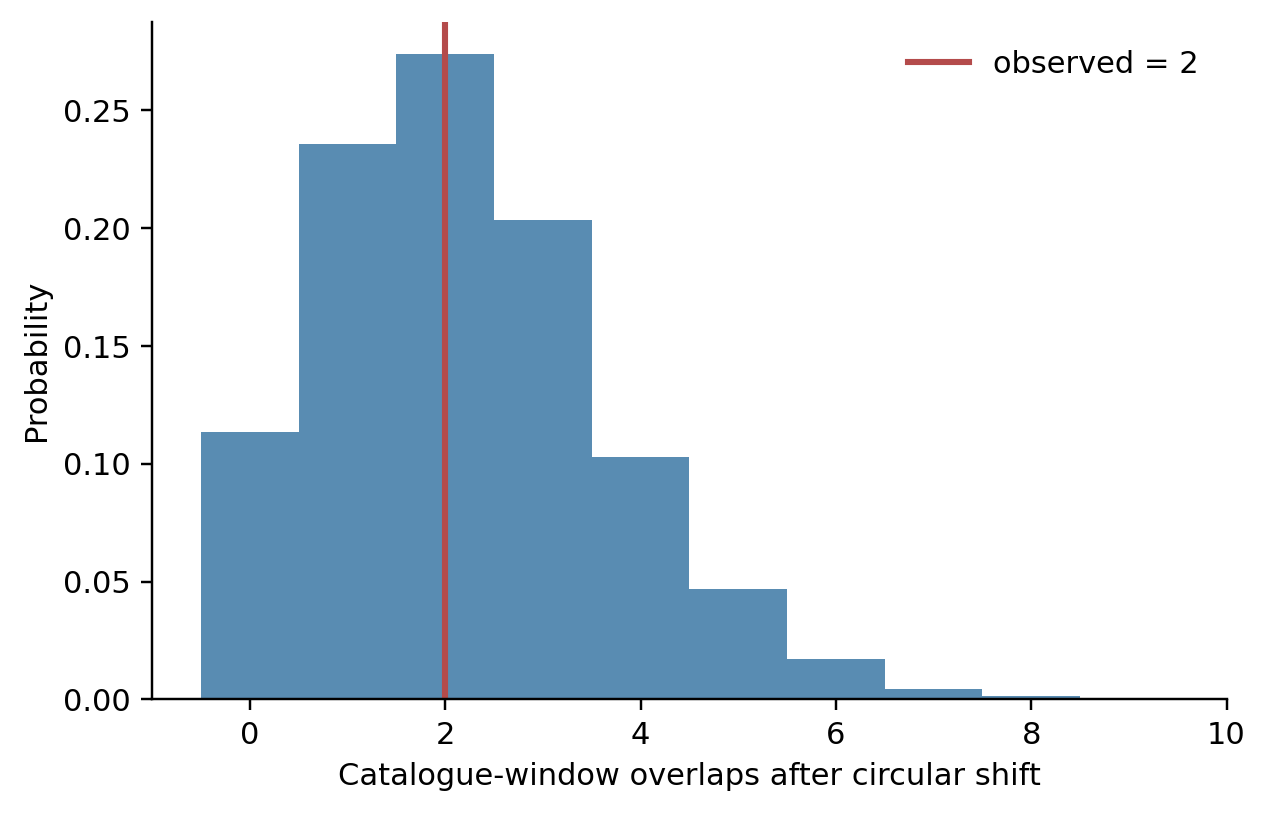
\includegraphics[width=\columnwidth]{fig_catalog_null_q64.png}
\caption{Catalogue-overlap circular-shift coverage proxy.  The observed two
any-detector overlaps are consistent with the null distribution and do not
measure catalogue recall.}
\label{fig:catalog-null}
\end{figure}

\subsection{Compact-binary injection controls}

We inject zero-spin, non-precessing IMRPhenomD waveforms into raw real vetoed
O4a noise for BBH $30+30\,M_\odot$, BBH $10+10\,M_\odot$, and NSBH
$10+1.4\,M_\odot$ at 100, 200, 400, 800, and 1,600\,Mpc.  The lower waveform
frequencies are 20, 25, and 30\,Hz, respectively.  With seed 42, each trial
draws right ascension and polarization uniformly, declination isotropically,
and inclination uniformly in $\cos\iota$; the two detector strains use their
own antenna responses and geocentric delays.  The merger is placed at the
analysis-window centre, and the otherwise identical uninjected H1/L1 segments
provide paired clean controls.  A successful trial requires finite strain in
both detectors and completion of injection, whitening, scoring, localization,
and coincidence; failed data fetches or invalid stretches are skipped rather
than counted as misses.  There are 25 successful trials per cell (375
injections).  For $30+30\,M_\odot$ at 100 and 200\,Mpc, the primary score
flags 23/25 and 12/25 trials, while end-to-end physical coincidence recovers
16/25 (Wilson 95\% interval 0.445--0.798) and 9/25
(0.202--0.555).  For $10+10\,M_\odot$, primary flagging is 22/25 and 14/25,
but coincidence is 12/25 and 0/25.  NSBH coincidence is zero in all tested
cells.  Native DSD disposition is detector- and distance-dependent rather than
a monotonic continuation of the primary score (Fig.~\ref{fig:cbc}).

\begin{figure*}[t]
\centering
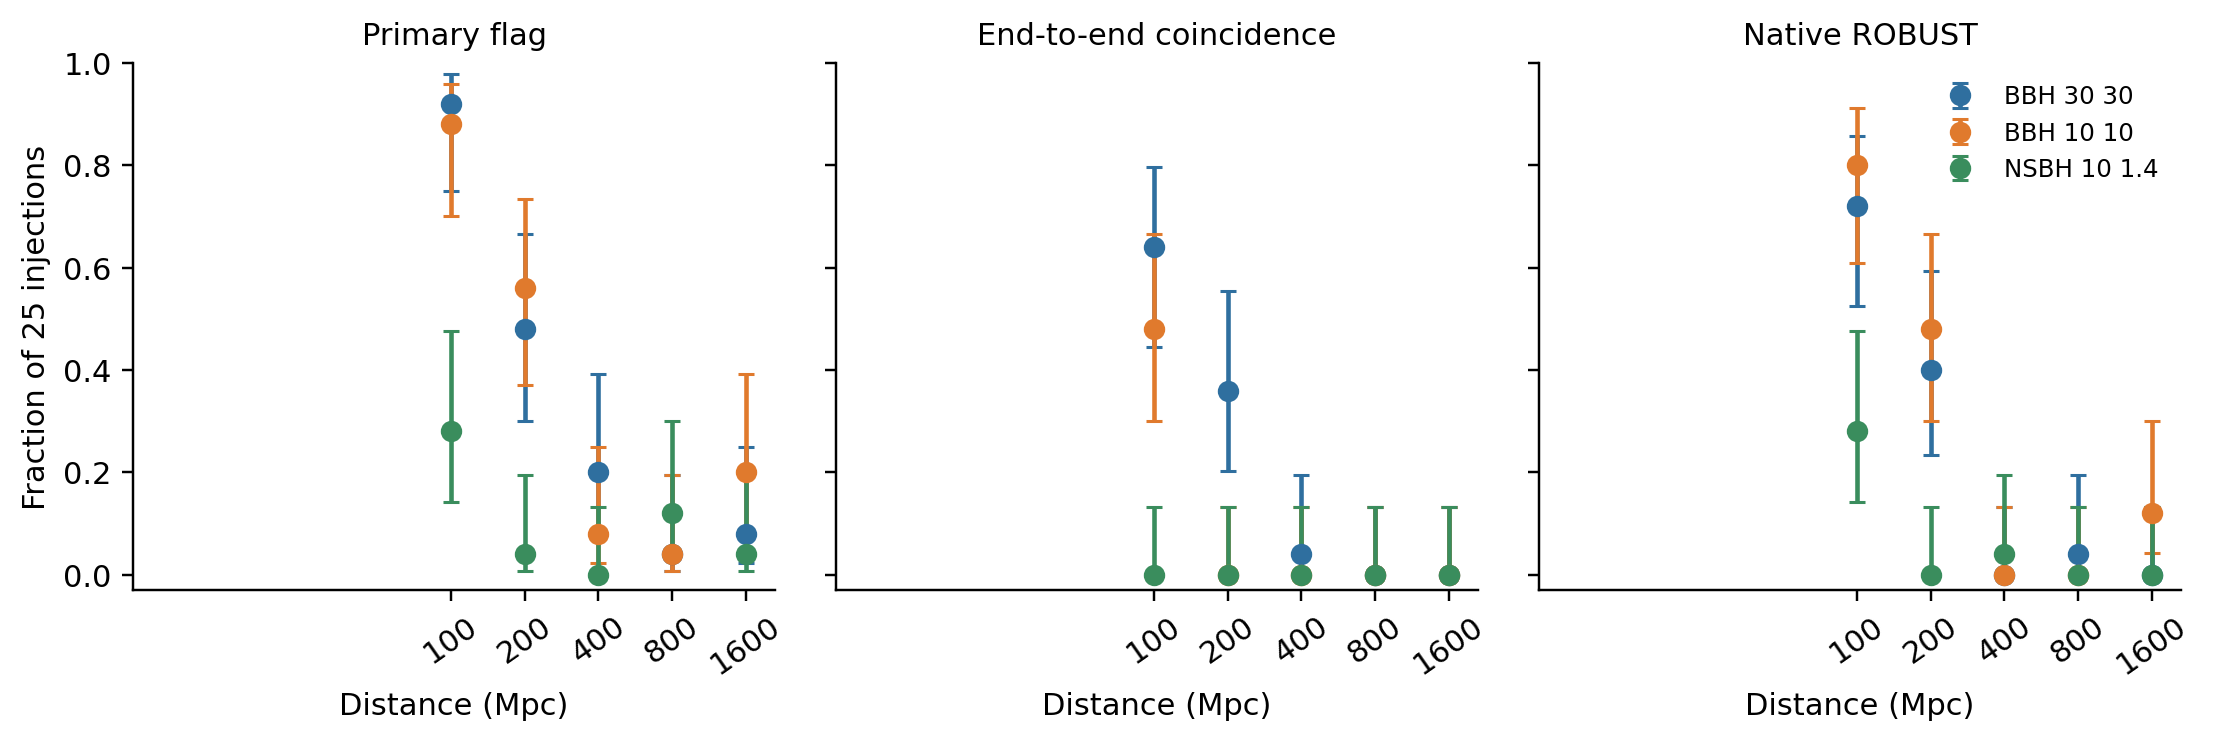
\includegraphics[width=0.94\textwidth]{fig_cbc_controls_q64.png}
\caption{Simulation-only compact-binary controls.  Points show the primary
flag, end-to-end physical coincidence, and maximum single-detector
\robust\ fraction; binomial error bars are Wilson 95\% intervals.  Each point
contains 25 successful injections into real O4a noise.}
\label{fig:cbc}
\end{figure*}

The simulation demonstrates morphology-dependent response and a tension
between historical novelty and native adaptation.  It is not an end-to-end
astrophysical efficiency: merger placement is known by construction, only one
zero-spin intrinsic point is tested per named system, and BNS
$1.4+1.4\,M_\odot$ is not measured
because its 31\,s waveform violates the current 32\,s safety margin.  We
therefore exclude BNS and make no CBC-complete or astrophysical-rate claim.

\section{Discussion}
\label{sec:discussion}

The coherent DSD removes one avoidable ambiguity---a mismatch between the
representation used to build the index and the one used to query it---but it
does not make the survivor label physically self-interpreting.  Three distinct
uncertainties remain.

First, the need for native adaptation is itself detector-dependent.  The
matched H1 experiment resolves an O3b--O4a score shift and a reduction after
native adaptation, whereas the corresponding L1 intervals include zero.
Native adaptation therefore cannot be described as universally correcting an
``O4a shift.''  Published O4a detector characterization provides plausible but
non-causal context: LHO transient noise was dominated by low-SNR 10--50\,Hz
features with a broadband source mitigated during O4a, whereas LLO transient
noise was dominated by seasonally varying, microseism-driven scattered light
\cite{soni2025}.  Our embedding-level experiment does not localize the
contributing bands or morphologies and therefore cannot attribute the measured
asymmetry to those mechanisms.  Where native adaptation is used, it also trades shift reduction against
absorption: a background index can regard a recurrent new morphology as normal
precisely because it is recurrent.  Candidate-vetoed sampling limits direct
circularity, but it cannot remove unflagged members of the same population.
The replicated three-morphology contamination experiment turns this concern
into a measurable, configuration-dependent failure mode.

Second, preprocessing and dictionary construction are part of the statistical
model, and the size of this effect is not marginal: correcting a single
representation mismatch, between the Q-range used to build the native index
and the Q-range used to query it, changed 4,676 of 10,372 paired dispositions,
close to half the historical catalogue. This magnitude means representation
contracts cannot be treated as metadata hygiene; they are load-bearing for the
reported taxonomy. The risk is mitigated but not eliminated: every dependent
artefact carries a stored SHA256 hash of its representation contract, and all
class-dependent analyses reject execution on a hash mismatch, but this closes
only the specific mismatch identified here, not the possibility of an
analogous one elsewhere in the pipeline. The moderate draw stability, $K$
dependence, and whitening-context sensitivity reported above are of a
different, smaller character and must not be read as bounding this larger
risk. A deterministic forward pass is not equivalent to a robust scientific
disposition.

Third, physical nulls must match the nuisance structure.  In PEM coherence,
time shifts do not control persistent spectral coupling; a quiet zero-lag null
reduces 48 apparent positives to 10 confirmed endpoints.  In catalogue
matching, a raw overlap count is uninterpretable without processed coverage
and a time-structured null.  In cross-detector tests, embedding similarity is
not a substitute for light-travel-consistent strain correlation.

These findings also delimit the relationship to astrophysical anomaly
searches.  DANTE produces a ranked candidate queue intended to support
detector-characterization triage and auxiliary investigation; this study does
not measure improvement in human or operational triage efficiency.  The present calibration cannot supply astrophysical
significance.  A future search-oriented system would need injection populations
covering its target sources, causal or training-period-only adaptation,
multi-detector coherence in the ranking statistic, and explicit false-alarm
calibration over searched livetime.

\section{Reproducibility and limitations}

All class-dependent analyses load the coherent Q64/Q64 taxonomy, validate the
index hash and Q-range, and reject missing
or non-finite scores. The complete repository suite contains 174 passing tests
and one platform-dependent skip.
A separate
fail-closed artefact audit checks ten named C2 stages and their upstream
calibration contracts.  The catalogue and PEM experiments have dedicated
input/output SHA256 manifests; new scans persist an append-only ledger of
successfully scored windows.

The main limitations are scientific rather than hidden execution failures.
The historical O4a scan lacks an exact successful-window ledger, five of 84
session--detector files calibrate their exploratory primary threshold on fewer
than 500 windows, and physical-coincidence missingness is not known to be
random; PEM uses only
publicly available, non-safety-certified channels; the C2 robustness study
emphasizes deliberately near-boundary samples, while the final robustness
study uses only 160 candidates per population; the absorption matrix is
synthetic and restricted to O4a L1, one peak amplitude and one prescribed
duration per morphology, three
morphologies, and three clustering seeds; the known-glitch controls are binary
O3b comparisons rather than O4a multiclass recall; the blind map has eight
trials per cell; and the CBC campaign excludes BNS.  The native index and
thresholds are O4a-specific, so another observing run requires new index
construction, calibration, and empirical validation.

\section{Conclusions}

A representation-coherent native calibration materially changes an
unsupervised O4a candidate taxonomy, but it does not convert statistical
novelty into a new glitch class.  Direct controls show that the measured
O3b--O4a shift and the effect of native adaptation differ between H1 and L1;
known-glitch separation also depends on morphology and detector.  The other
measured failure modes are population-dependent sensitivity to the
native-background draw, clustering seed, dictionary size, and whitening
context; synthetic absorption of recurrent anomalies; and a
morphology-dependent low-Q blind region.  Physical and catalogue controls
resolve no \robust-class PEM enrichment or catalogue overlap excess.  The
conservative cross-detector max-shift screen is non-exchangeable and supports
neither a tail-count $p$-value nor a discovery claim.  Compact-binary controls
further show that run-native
adaptation can suppress signals flagged by a historical reference.

For unsupervised GW detector characterization, native recalibration can be
necessary when a shift is measured, but it is not neutral.  Credible discovery requires publishing the
representation contract, calibration populations, negative controls, and
failure modes together with the candidate list -- concretely, treating
representation, reference population, calibration population, and physical
null as four linked, separately checkable objects, rather than as implementation
detail.

\section*{Data availability}

Public O4a strain and auxiliary data are available from GWOSC
\cite{gwosc_aux_o4,gwosc_o4a_release}.  DANTE 3.7.0 is archived as a versioned
software snapshot on Zenodo \cite{dante_zenodo}.  The representation-versioned
result tables, per-trial outputs, environment records, SHA256 manifests, and
verification tools supporting this study are archived separately in the DANTE
v6 reproducibility and validation evidence dataset
\cite{dante_v6_evidence}.  Their repository paths and provenance are enumerated
in the accompanying lab notebook.

\section*{Code availability}

The analysis code, command reference, tests, and paper-figure generator are
available in the DANTE repository associated with \cite{dante_zenodo}.  A new
run requires run-specific native indices, thresholds, and null calibrations.

\section*{Acknowledgements}

OpenAI Codex (GPT-5, service version accessed July--August 2026) was used for
language editing, consistency checks
between manuscript claims and saved artefacts, and assistance with test and
figure code.  It was not used to generate scientific data.  The author
designed the study, executed the analyses, checked the artefacts and
references, and accepts responsibility for the manuscript.

\section*{Funding}

This research received no external funding.

\section*{Competing interests}

The author declares no competing interests.

\section*{Author contributions}

L.C. conceived the study, developed the software, performed the analyses,
interpreted the results, and wrote and reviewed the manuscript.

\appendix

\section{Representation-contract ablation}

Table~\ref{tab:transition} reports the complete transition from the
cross-representation Q32-index/Q64-query ablation to the coherent Q64/Q64
disposition.  The mismatched columns remain in the released table for
auditability; all scientific analyses use the coherent columns through the
taxonomy contract.

\begin{table}[htbp]
\centering
\caption{DSD representation-ablation matrix.  Rows are the mismatched
Q32/Q64 disposition and columns the coherent Q64/Q64 disposition.  The single
UNKNOWN row was
coherently evaluated as \background.}
\label{tab:transition}
\begin{tabular}{lrrr}
\toprule
Q32/Q64 & \robust & \ambiguous & \background \\
\midrule
\robust & 2,914 & 14 & 9 \\
\ambiguous & 1,666 & 68 & 39 \\
\background & 1,759 & 1,188 & 2,714 \\
UNKNOWN & 0 & 0 & 1 \\
\bottomrule
\end{tabular}
\end{table}

\section{Numerical validation matrix}

Table~\ref{tab:validation} consolidates the fixed-before-execution and
load-bearing validation questions that bound the interpretation of the main
results.

\begin{longtable}{@{}
  >{\raggedright\arraybackslash}p{0.20\textwidth}
  >{\raggedright\arraybackslash}p{0.47\textwidth}
  >{\raggedright\arraybackslash}p{0.25\textwidth}
  @{}}
\caption{Fixed-before-execution or load-bearing validation questions and their coherent
outcomes.  Negative results are retained because they bound interpretation.}
\label{tab:validation}\\
\toprule
Question & Design & Result \\
\midrule
\endfirsthead
\toprule
Question & Design & Result \\
\midrule
\endhead
Background-draw stability & Four independent 1,300-segment dictionaries; 160
near-boundary candidates & mean/min $\rho=0.674/0.515$ \\
Final robustness replication & Eight draws, five clustering seeds, and four
$K$ values; fixed near-boundary and unconditioned pools & mean $\rho=0.903$--$0.954$
near boundary; $0.977$--$0.988$ unconditioned \\
Cross-run domain shift & Matched O3b/O4a clean windows; $K=56$ control
dictionaries, same O3b index, native adaptation, and out-of-fold run probe & H1 shift/adaptation resolved; L1
differences include zero \\
Known-glitch construct control & 30 labelled O3b examples per
morphology/detector versus 40 clean windows & strong Scattered Light/Koi Fish;
weak L1 Blip separation \\
Dictionary size & $K=512,1024,1216,2048$ on the same candidates and cached
tokens & $\rho$ vs production $=0.753,0.768,0.943$ \\
Representation comparators & PCA residual, total spectral energy, and a
detector-specific convolutional autoencoder & AUC $=0.436,0.544,0.473$ \\
Whitening reproduction & Recompute pad-4 score for 60 retained candidates &
maximum $|\Delta A|=6.85\times10^{-7}$; 60/60 pass \\
Whitening sensitivity & Pads 16, 64, 128\,s with fixed and recalibrated
thresholds & flips 37--40\% fixed; 63--70\% recalibrated \\
Absorption & Three morphologies, three seeds, prevalence sweep, and same-size
background control & joint-rule crossings: Blip 2--5\%, Koi Fish 10\%,
Scattered Light 5\% \\
Blind map & $5\times8$ centred sine-Gaussian grid; SNR 20; $n=8$ per cell &
mean 26.3\% at $Q\le64$, 48.8\% at $Q>64$ \\
Graph cohesion & Same $D_{\rm cut}=0.25$ applied to all classes and native
background & statistic saturated; non-discriminating \\
Inter-session recurrence & Top pairs and neighbour-session span versus shuffled
labels & no positive recurrence resolved \\
Physical coincidence & 8,806 measured of 10,429 candidate windows; pooled
per-event maxima from 4--8 shifts & 13 exceed $\tau_{\rm cc}$; conservative,
non-exchangeable screen; no tail-count $p$-value \\
PEM class association & Family-wise time-shift and quiet zero-lag nulls &
2/26 vs 7/93; OR 1.02; $p=1.000$ \\
Catalogue overlap & 135 GWTC events; coverage proxy; 10,000 circular shifts &
2 observed; null $2.190\pm1.467$; $p=0.651$ \\
CBC response & Three systems, five distances, 25 completed injections per cell
& primary, coincidence, and native responses differ; Wilson intervals reported \\
\bottomrule
\end{longtable}

\section{Requirements for another observing run}

The code separates run-named output directories and representation-versioned
indices, but scientific portability is not established by changing a command
line label.  Reprocessing historical data or analysing a future run requires:

\begin{enumerate}
\item explicit GPS bounds and detector participation for the run;
\item a declared data-quality policy and strain availability audit;
\item a new candidate scan and exact successful-window ledger;
\item a candidate-vetoed run-native index with representation metadata;
\item independent run-native threshold populations and temporal bootstrap;
\item time-shift coincidence and catalogue nulls over the new livetime;
\item an auxiliary-channel inventory and new family-wise PEM calibration where
      public data permit it; and
\item end-to-end software tests followed by a real-data smoke test.
\end{enumerate}

The discovery/aggregation path is tested hermetically for O4a and O3b.  O2,
O3a, and future O5 results are not claimed as scientifically validated in this
paper.  This distinction prevents software parameterization from being
misreported as observational validation.

\section{Validation safeguards and excluded interpretations}

Four implementation safeguards are load-bearing for interpretation.  Candidate
timestamps identify the scored 32\,s interval rather than the beginning of the
padded fetch.  Physical coincidence maps localized patches to the correct
strain axes and light-travel window.  Every class-dependent result resolves a
coherent Q64/Q64 representation contract.  Centred injection studies reproduce
the canonical pad-4 stored-score anchor before any preprocessing comparison.

The evidence does not support a universal DSD-absorption threshold, invariant
ranking under background draw or dictionary size, significant PEM enrichment
of \robust\ candidates, survey-wide whitening stability, a universal high-Q
blind boundary, CBC-complete efficiency, catalogue recall, transferable rate
limits, or a new physical glitch class.

\bibliographystyle{unsrt}
\bibliography{references}

\end{document}
